\documentclass[11pt,          % font size: 11pt or 12pt
               phd,           % degree:    ms or phd
               onehalfspacing % spacing: onehalfspacing or doublespacing
               ]{ncsuthesis}

%%----------------------------------------------------------------------------%%
%%------------------------------ Import Packages -----------------------------%%
%%----------------------------------------------------------------------------%%

\usepackage{booktabs}  % professionally typeset tables
\usepackage{amsmath}%,amssymb,amsfonts}
\usepackage{textcomp}  % better copyright sign, among other things
%\usepackage{xcolor}
\usepackage{lipsum}    % filler text
\usepackage{subfig}    % composite figures

%%ORTIZ PACKAGES


%%%%%%%%%%%%%%%%%%%%%%%%%%%%%%%%%%%%%%%%%%
%%%%%%%%%%% Old bibliography commands
%%%%%%%%%%%%%%%%%%%%%%%%%%%%%%%%%%%%%%%%%%5
%\usepackage[super,sort&compress,comma,square,authoryear]{natbib} %\cite command %Added by Ortiz

%use the following line with plainnat
%\usepackage[super,sort&compress,comma,square,numbers]{natbib} %\cite command %Added by Ortiz
%\usepackage{natbib}

%\usepackage[style=alphabetic,natbib=true,backend=bibtex
%sorting=nyt,firstinits=true,isbn=false,doi=false,url=false]{biblatex} %couldn't get backend=biber to work

%\usepackage{filecontents}

%\bibliography{Ortiz-thesis2}
%\bibliographystyle{plain}


%%%%%%%%%%%%%%%%%%%%%%%%%%%%%%%%%%%%%%%%%%
%%%%%%%%%%% Hack for alphanumeric bibliography
%%%%%%%%%%%%%%%%%%%%%%%%%%%%%%%%%%%%%%%%%%5
\RequirePackage[
			style=alphabetic,%numeric-comp,%authoryear-comp,%
			sorting=nyt,%ynt					
			hyperref=true, %	
			firstinits=true,%
			backend=bibtex,
			natbib=true,
			url=false,
			isbn=false,
			maxnames=2, %for et al to be used
			maxalphanames=1, %to avoid printing a + for every et al in the abbreviation
			doi=false]{biblatex}		
			

%needed to do et al after two names
%http://tex.stackexchange.com/questions/44048/use-et-al-in-biblatex-custom-style
\renewcommand*{\finalnamedelim}{\addspace\&\space}

%Simplify abbreviation (the default uses either one or two authors and it indicates et al with a +)
%The following five lines make it so that only the first author is used in the abbreviation
%http://tex.stackexchange.com/questions/27956/label-only-from-first-author
\renewcommand*{\labelalphaothers}{}
    \renewcommand*{\intitlepunct}{}
    \DefineBibliographyStrings{german}{in={}}
    \DefineBibliographyStrings{english}{in={}}
    \DeclareNameAlias{sortname}{last-first}
    \DeclareNameAlias{default}{last-first}
	
%\AtEveryCitekey{\ifciteseen{}{\defcounter{maxnames}{99}}} %authoryear			
\DeclareFieldFormat[article,periodical]{volume}{\mkbibbold{#1}}
\makeatletter

\newrobustcmd*{\parentexttrack}[1]{%
  \begingroup
  \blx@blxinit
  \blx@setsfcodes
  \blx@bibopenparen#1\blx@bibcloseparen
  \endgroup}

\AtEveryCite{%
  \let\parentext=\parentexttrack%
  \let\bibopenparen=\bibopenbracket%
  \let\bibcloseparen=\bibclosebracket}

\makeatother
\renewcommand{\cite}[1]{\parencite{#1}}


\renewbibmacro{in:}{%
  \ifentrytype{article}{}{%
  \printtext{\bibstring{in}\intitlepunct}}}
  
\AtEveryBibitem{\clearfield{month}}

\AtEveryBibitem{\clearfield{language}}
%%%%%%%%%%%%%%%%%%%%%%%%%%%%%%%%%%%%%%%%%%%%%

%\addbibresource{Ortiz-thesis2.bib}
%\addbibresource{Ortiz-thesisURL.bib}
\addbibresource{bigfatnoob-thesis.bib}

 \defbibheading{myheading}[BIBLIOGRAPHY]{
 \chapter*{#1}
 %\centerline{\bf{#1}}
 \markboth{#1}{#1}}

%\usepackage{amsmath,amssymb,amsfonts} %amssymb and amsfonts cannot be used in conjunction with mdput
%\usepackage{graphicx,subfig}% Include figure files
\usepackage{dcolumn}% Align table columns on decimal point
\usepackage{bm}% bold math
%\usepackage{hyperref}% add hypertext capabilities
%\usepackage{hypernat}% make hyperref and natbib work together
\usepackage{cancel}
\usepackage{verbatim}% multiline commenting
\usepackage{ifthen}
\usepackage{url}
\usepackage{sectsty}
\usepackage{balance} 
%\usepackage{caption}
\usepackage{graphicx} %eps figures can be used instead
\usepackage{lastpage}
\usepackage[format=plain,justification=RaggedRight,singlelinecheck=false,font=small,labelfont=bf,labelsep=space]{caption} 
\usepackage{fancyhdr}
\pagestyle{fancy}

%http://tex.stackexchange.com/questions/100817/error-when-using-bc-from-abbrevs-in-caption
%Getting BC
\usepackage{abbrevs}
\usepackage{etoolbox}
\robustify{\DateMark} % after having loaded abbrevs

\usepackage{units} %Needed to solve bug from citation Hydrodynamics in 21/2 dimensions
%see http://www.latex-community.org/viewtopic.php?f=5&t=989

\usepackage[sharp]{easylist} %used for brainstorming purposes 
%\usepackage{mathabx} % used for \Asterisk for convolution %conflicts with \widering

%compile on single pass
%\usepackage[backend=biber,...]{biblatex}


%%%%%%%%%%%%
%%% Hack to make chapters start on odd pages
% http://tex.stackexchange.com/questions/73591/how-to-have-a-blank-even-page-before-every-chapter
%%%%%%%%%%%%
%\newcommand{\ensureoddstart}{\checkoddpage\ifoddpage\else\newpage\mbox{}\fi}
%\newcommand{\ensureoddstart}{}


%%%Fancy tables
%http://tex.stackexchange.com/questions/94032/fancy-tables-in-latex
\usepackage[table]{xcolor}
\usepackage{array,booktabs}
\usepackage{colortbl}
\newcolumntype{L}{@{}>{\kern\tabcolsep}l<{\kern\tabcolsep}}



%%%%%%%%%%
%%%%% Hack to allow more levels in outline
%%%%%%%%%%
%\setcounter{secnumdepth}{5}
%\setcounter{tocdepth}{5} %may violate ETD
%Usage http://pleasemakeanote.blogspot.com/2010/06/how-to-activate-subsubsubsection-in.html
%\section{} % level 1
%\subsection{} % level 2
%\subsubsection{} % level 3
%\paragraph{} % level 4 - equivalent to subsubsubsection
%\subparagraph{} % level 5

%http://tex.stackexchange.com/questions/60209/how-to-add-an-extra-level-of-sections-with-headings-below-subsubsection
\usepackage{titlesec}

\setcounter{secnumdepth}{4}

\titleformat{\paragraph}
{\normalfont\normalsize\bfseries}{\theparagraph}{1em}{}
\titlespacing*{\paragraph}
{0pt}{3.25ex plus 1ex minus .2ex}{1.5ex plus .2ex}

%%%%%%%%%%%%%%%%%%%%%%%%%%
%%%% Hack for containing figures within sections
%%%%%%%%%%%%%%%%%%%%%%%%%%%%
%http://ctan.org/pkg/placeins
\usepackage{placeins}
%De�fines a \FloatBar�rier com�mand, be�yond which floats may not pass; use�ful, for ex�am�ple, to en�sure all floats for a sec�tion ap�pear be�fore the next \sec�tion com�mand.

%%%Hack for centering all figures
%\makeatletter
%\g@addto@macro\@floatboxreset\centering
%\makeatother

%%----------------------------------------------------------------------------%%
%%---------------------------- Formatting Options ----------------------------%%
%%----------------------------------------------------------------------------%%
%%

%% -------------------------------------------------------------------------- %%
%% Disposition format -- any titles, headings, section titles
%%  These formatting commands affect all headings, titles, headings,
%%  so sizing commands should not be used here.
%%  Formatting options to consider are
%%     +  \sffamily - sans serif fonts.  Dispositions are often typeset in
%%                    sans serif, so this is a good option. 
%%     +  \rmfamily - serif fonts
%%     +  \bfseries - bold face
%\dispositionformat{\sffamily\bfseries}   % bold and sans serif
\dispositionformat{\bfseries}            % bold and serif

%% -------------------------------------------------------------------------- %%
%% Formatting for centered headings - Abstract, Dedication, etc. headings
%%  This is where one might put a sizing command.
%%  \MakeUppercase can be used to typeset all headings in uppercase.
\headingformat{\large\MakeUppercase}   % All letters uppercase
%\headingformat{\large}                % Not all uppercase
%\headingformat{\Large\scshape}        % Small Caps, used with serif fonts.

%% Typographers recommend using a normal inter-word space after
%% sentences. TeX's default is to add an wider space, but \frenchspacing
%% gives a normal spacing. Comment out the following line if you prefer
%% wider spaces between sentences.
\frenchspacing


%% -------------------------------------------------------------------------- %%
%%  Optional packages
%%    A number of compatible packages to improve the look and feel of
%%    your document are available in the file optional.tex 
%%    (For example, hyperlinks, fancy chapter headings, and fonts)
%% To use these options, uncomment the next line and see optional.tex
%%  Optional Packages to consider.   These packages are compatible with
%%    ncsuthesis.  

%% -------------------------------------------------------------------------- %%
%% Fancy chapter headings
%%  available options: Sonny, Lenny, Glenn, Conny, Rejne, Bjarne
%\usepackage[Sonny]{fncychap}
\usepackage[Rejne]{fncychap}

%%----------------------------------------------------------------------------%%
%% Hyperref package creates PDF metadata and hyperlinks in Table of Contents
%%  and citations.  Based on feedback from the NCSU thesis editor, 
%%  the links are not visually distinct from normal text (i.e. no change
%%  in color or extra boxes).
\usepackage[
  pdfauthor={Carlos Pompeyo Ortiz},
  pdftitle={Rigidity of Microsphere Heaps},
  pdfcreator={pdftex},
  pdfsubject={NC State ETD Thesis},
  pdfkeywords={microfluidics, hard sphere, jamming, suspension, rigidity, friction, microscopy},
  colorlinks=true,
  linkcolor=black,
  citecolor=black,
  filecolor=black,
  urlcolor=black,
]{hyperref}


%% -------------------------------------------------------------------------- %%
%% Microtype - If you use pdfTeX to compile your thesis, you can use
%%              the microtype package to access advanced typographic
%%              features.  By default, using the microtype package enables
%%              character protrusion (placing glyphs a hair past the right 
%%              margin to make a visually straighter edge)
%%              and font expansion (adjusting font width slightly to get 
%%              more favorable justification).
%%              Using microtype should decrease the number of lines
%%              ending in hyphens.
\usepackage{microtype}


%%----------------------------------------------------------------------------%%
%% Fonts 

%% ETD guidelines don't specify the font.  You can enable the fonts
%%  by uncommenting the appropriate lines.  Using the default Computer 
%%  Modern fonts is *not* required.  A few common choices are below.
%%  See http://www.tug.dk/FontCatalogue/ for more options.

%% Serif Fonts -------------------------------------------------
%%  The four serif fonts listed here (Utopia, Palatino, Kerkis,
%%  and Times) all have math support.


%% Utopia
\usepackage[T1]{fontenc}
\usepackage[adobe-utopia]{mathdesign}

%% Palatino
%\usepackage[T1]{fontenc}
%\usepackage[sc]{mathpazo}
%\linespread{1.05}

%% Kerkis
%\usepackage[T1]{fontenc}
%\usepackage{kmath,kerkis}

%% Times
%\usepackage[T1]{fontenc}
%\usepackage{mathptmx}


%% Sans serif fonts -------------------------

%\usepackage[scaled]{helvet}  % Helvetica
%\usepackage[scaled]{berasans} % Bera Sans

%solve bug from fancyhdr in optional
%http://nw360.blogspot.com/2006/11/latex-headheight-is-too-small.html
\setlength{\headheight}{14pt}

%%----------------------------------------------------------------------------%%
%%---------------------------- Content Options -------------------------------%%
%%----------------------------------------------------------------------------%%
%% Size of committee: 3, 4, 5, or 6 -- this number includes the chair
\committeesize{4}

%% Members of committee
%%  Each of the following member commands takes an optional argument
%%   to specify their role on the committee.
%%  For co-chairs, use the commands:
%%      \cochairI{Doug Dodd}
%%      \cochairII{Chris Cox}
%%
\chair{Doug Dodd}
\memberI{Alex Anderson}
\memberII{Bobby Brown}
\memberIII{Chris Cox}   % unnecessary if committeesize=3
\memberIV{Fred Ford}    % unnecessary if committeesize=3 or 4
\memberV{Edna Everitt}  % unnecessary if committeesize=3, 4, or 5


%% Student writing thesis, \student{First Middle}{Last}
\student{John Mark}{Smith} % a full middle name
%\student{John M.}{Smith} % a middle initial

%% Degree program
\program{Physics}

%% Thesis Title
%%  Keep in mind, according to ETD guidelines:
%%    +  Capitalize first letter of important words.
%%    +  Use inverted pyramid shape if title spans more than one line.
%%
%%  Note: To break the title onto multiple lines, use \break instead of \\.
%\thesistitle{A North Carolina State University Sample \LaTeX{} Thesis \break 
%with a Title So Long it Needs a Line Break}
\thesistitle{A North Carolina State University Sample \LaTeX{} Thesis \break 
with a Title So Long it Needs a Line Break}

%% Degree year.  Necessary if your degree year doesn't equal the current year.
%\degreeyear{1995}


%%----------------------------------------------------------------------------%%
%%---------------------------- Personal Macros -------------------------------%%
%%----------------------------------------------------------------------------%%

%% A central location to add your favorite macros.

%% A few examples to get you started.
\newcommand{\uv}[1]{\ensuremath{\mathbf{\hat{#1}}}}
\newcommand{\bo}{\ensuremath{\mathbf{\Omega}}}
\newcommand{\eref}[1]{Eq.~\ref{#1}}
\newcommand{\fref}[1]{Fig.~\ref{#1}}
\newcommand{\tref}[1]{Table~\ref{#1}}
\newcommand{\del}{\nabla}
\renewcommand{\exp}[1]{e^{#1}}
\newcommand{\Conv}{\mathop{\scalebox{1.5}{\raisebox{-0.2ex}{$\ast$}}}}%


\usepackage{color}
%\newcommand{\NEW}[1]{\textcolor{blue}{#1}}
\newcommand{\NEW}[1]{#1}
\newcommand{\COMMENT}[1]{\textcolor{green}{#1}}


\newcommand{\NOTER}[1]{\textcolor{orange}{#1}}
\newcommand{\NOTEC}[1]{\textcolor{blue}{#1}}
\newcommand{\NOTEK}[1]{\textcolor{magenta}{#1}}

\newcommand{\mum}{\ensuremath{{\mu}\text{m}}}

%This makes it so that you can add short paths in your .tex by including the folders where you store your images in the search path
\graphicspath{{./Chapter-1/figs/}{./Chapter-2/figs/}{./Chapter-3/figs/}}%{./Chapter-4/figs/}{./Chapter-5/figs/}{./Chapter-6/figs/}}


%%---------------------------------------------------------------------------%%
\usepackage{calc}
%% Capital letter height
\newlength{\chaptercapitalheight}
\settoheight{\chaptercapitalheight}{D}
\newlength{\chapterfootskip}
\setlength{\chapterfootskip}{\chaptercapitalheight}
\addtolength{\chapterfootskip}{2\baselineskip}
\addtolength{\chapterfootskip}{0.5ex}  % A little extra space to ensure there are 2 full double spaced lines
%\def\chapterfootskipnum{\chapterfootskip}
\renewcommand{\listfigurename}{LIST OF FIGURES}
\renewcommand{\listtablename}{LIST OF TABLES}
\renewcommand{\bibname}{BIBLIOGRAPHY}

%\renewcommand{\cfttoctitlefont}{\centering\ncsu@headingformat}


%http://tex.stackexchange.com/questions/47184/height-of-figure-caption-textheight
\newlength\graphht
\newcommand\calculategraphicstargetheight[1]{%
     \setlength\graphht{\textheight 
                       -\parskip
                       -\abovecaptionskip -\belowcaptionskip
                       -(12pt * #1) % assuming baselineskip of 12pt in caption
                       -\chapterfootskip
                       }}

%\usepackage{titlesec}

%landscape support in fancyhdr from http://tex.stackexchange.com/questions/9071/how-to-translate-and-rotate-the-heading-of-landscaped-pages
\usepackage{pdflscape}
\usepackage{tikz}
\fancypagestyle{lscapedplain}{%
  \fancyhf{}
  \fancyfoot{%
    \tikz[remember picture,overlay]
      \node[outer sep=1cm,above,rotate=90] at (current page.east) {\thepage};}
\renewcommand{\headrulewidth}{0pt} 
\renewcommand{\footrulewidth}{0pt}
}

                      
\begin{document}
\pagestyle{plain}
%%---------------------------------------------------------------------------%%
\frontmatter

%% ------------------------------ Abstract ---------------------------------- %%
\begin{abstract}
Making decisions amongst a set of choices is a primary need of complicated goal models with multiple possible choices. Many a time, business analysts fail in selecting different sets of decisions which result in satisfying multiple stakeholders' goals with some optimal trade-offs between possibly conflicting ones. Most quantitative requirement engineering goal models support such activities by describing alternative design paths with different impact on the levels of goal satisfaction specified in the terms of measurable objective functions. This thesis proposes a framework called DEBRA, to identify different sets of optimal decisions that satisfy conflicting goals using Differential Evolution, a multi-objective optimization algorithm. The experimental study was conducted on two types of requirements engineering goal models; i* and Analytic Hierarchy Process(AHP). The work further highlights a probability based method to identify the most significant decisions and justifies that in most software models, there exists prominent decisions such that if set to their optimum value, it can lead to significant reduction in the cumulative engineering cost of the most requirement engineering goal models.
\end{abstract}

%% ---------------------------- Copyright page ------------------------------ %%
%% Comment the next line if you don't want the copyright page included.
\makecopyrightpage

%% -------------------------------- Title page ------------------------------ %%
\maketitlepage

%% -------------------------------- Dedication ------------------------------ %%
\begin{dedication}
 \centering
 \TODO{Write Dedication}
\end{dedication}

%% -------------------------------- Biography ------------------------------- %%
\begin{biography}
\TODO{Write Biography}
\end{biography}

%% ----------------------------- Acknowledgements --------------------------- %%
\begin{acknowledgements}
I would like to thank my advisor for his help.
\end{acknowledgements}


\thesistableofcontents

\thesislistoftables

\thesislistoffigures

%%---------------------------------------------------------------------------%%
\mainmatter



\pagestyle{fancy}
\newgeometry{margin=1in,lmargin=1.25in,footskip=\chapterfootskip, includehead, includefoot}
\chapter{INTRODUCTION}
\label{chap-one}
Let's start with a few paragraph basics, here is how to make \textbf{bold}, 
and \textit{italics}, and \emph{emphasized}.  Let's say you need to cite 
something in your references, simply type \verb^\cite{key}^, which produces
\cite{einstein1935particle}.  
Some other references are \cite{golub1996matrix} and 
\cite{larsen1974asymptotic}.
Some \LaTeX{} compilers 
require a second compilation for citations and references 
to be sorted and matched properly in the resulting document.  

Here is a quotation:
\begin{quotation}
Alice, Bob and Carol are boring.  Who would even want to know their secret?
\end{quotation}

Let's say we need to make a list, try this on for size
\begin{enumerate}
  \item NCSU is great
  \item I like NCSU
  \item I really hope I can find a job when I graduate!
\end{enumerate} 

\section{Math enviroments}
\subsection{Equations}

There are many different ways to write equations, for example we could put 
$a^2 + b^2 = c^2$ directly into a sentence.  Or we could use the equation 
enviroment and do 
%
\begin{equation}
  a^2+b^2=c^2.
  \label{eq:one}
\end{equation} 
And from here we can later reference it by simply doing typing 
\verb^\ref{label}^, which gives \ref{eq:one}.  However, defining and using
equation and figure reference macros will ensure that the equation
references are consistent, instead of having Eq.~(1), Equation 3, Eqn 4
scattered through the thesis.  This template file defines \verb^\eref^
and \verb^\fref^ for this purpose. You can modify the macros to your liking
in the \texttt{YourName-thesis.tex} file.
For example, the command \verb^\eref{label}^ gives \eref{eq:one}.


If you don't need to reference an equation you may simply do this 
\[
  a^2 + b^2 = c^2.
\]

For Greek letters you must go to the math enviroments, for example 
$\alpha$, $\beta$, and $\gamma$.  Let's look at equations that cover 
multiple lines, none of these equations may be true or mean anything, but so 
that the reader can get some ideas.  In addition I will use some other useful 
notations like subscripts, superscripts, fractions, etc.  One important item 
of note is that one uses the ``ampersand" symbol to line up equations 
(also look at how I used quotations).
%
\begin{eqnarray}
\gamma_1 & = & \alpha^{\beta} + \psi_0 \frac{\psi_1}{\psi_2+\psi_3} \label{eq.two} \\
& = & \beta_1 + \beta_2 + \ldots + \beta_k \nonumber\\
& \rightarrow & E(\gamma_2) 
\end{eqnarray}

Alternatively, one can specify a slightly different enviroment if none of 
the equations need to be numbered.  Remember that if you are planning on 
referring to them later on, you must use a ``label" statement.
%
\begin{eqnarray*}
\gamma_1 & = & n^{-1/2} \displaystyle \sum_{i=1}^n \left[h(X_i,\beta_0)-E\{h(X_i,\beta_0)\}\right]\\
& \rightarrow & \hat q \pm \frac{\partial \gamma_2}{\partial \beta}. 
\end{eqnarray*}  
Lastly there may be times in which you want to use a non-italicized word 
your formula, such as an indicator function that may look like this 
$\mbox{I}\{\mu_i(1,\beta)>\mu_i(0,\beta)\}$ , if so just use the 
``mbox" statement.


You could use a multiline equation for long equations.  The environment
is \texttt{multline}.  Insert \verb^\\^ for line breaks.

\begin{multline*}
\bo \cdot \vec{\nabla} \psi(\vec{r},\bo ,E) + \Sigma_t(\vec{r},E)\psi(\vec{r},\bo ,E) = \\
  \int_{4\pi} d\bo' \int_0^{\infty} dE' \, \Sigma_s(\vec{r},\bo'\to\bo,E'\to E)\psi(\vec{r},\bo',E') + Q(\vec{r},\bo ,E),
\end{multline*}


we operate with $\displaystyle\int_{0}^{\infty}\left(\,\cdot\,\right) dE$
to obtain
\begin{multline*}
  \bo \cdot \vec{\nabla} \tilde{\psi}(\vec{r},\bo)
  + \Sigma_t(\vec{r})\tilde{\psi}(\vec{r},\bo) = \\
  \int_{4\pi} d\bo' \int_0^{\infty} dE' \, \psi(\vec{r},\bo',E')
  \left [ \int_{0}^{\infty} dE \, \Sigma_s(\vec{r},\bo'\to\bo,E'\to E)
  \right ] + \tilde{Q}(\vec{r},\bo),
\end{multline*}


\chapter{BACKGROUND}
\label{chap:bg}

\section{Goal Models}
\label{sec:bg:gm}
Goal Models are used in representing one or more goals. These goals are obtained from a system or its stakeholders. Goals often have relationships to other goals describing its impact or how they can be achieved. The primary aim of a goal model is to enhance the likelihood of a system's success by warranting that the software has a significant role in a complex socio-technical system. To augment this goal models allow explicit consideration of the system or its stake holders in the Requirements Engineering Process, there by allowing business analysts to assure that all the required goals are satisfied and all the proposed design alternatives or feature decisions satisfy the domain requirements. Goal Modeling is applied in multiple industrial systems like air traffic management \cite{maiden04}, non-profit organizations \cite{horkoff09} and health care domains \cite{anY09}. There are multiple goal modeling frameworks, techniques and methodologies. The remaining paragraphs in this section highlight few popular goal modeling frameworks.

\subsection{KAOS}
\label{subsec:bg:gm:kaos}
KAOS(\textit{\textbf{K}nowledge \textbf{A}cquisition in aut\textbf{O}mated \textbf{S}pecification}) is one of the first proposed Goal Modeling approaches \cite{van09} and is popular in eliciting, modelling and reasoning system requirements. The KAOS model contains two primary components, \textit{Goals} \& \textit{Agents}. Goals are prescriptive statements of intent that the system should satisfy through the cooperation of its agents, while agents are active system components playing specific roles in the satisfaction of goals. Goals are further refined into sub-goals through \textit{AND/OR} dependencies.
\begin{itemize}
    \item \textbf{AND}: Satisfaction of all of the sub-goals ensures satisfaction of the parent goal.
    \item \textbf{OR}: Satisfaction of either of the sub-goals ensures satisfaction of the parent  goal.
\end{itemize}

\begin{figure}[hbtp]
    \centering
    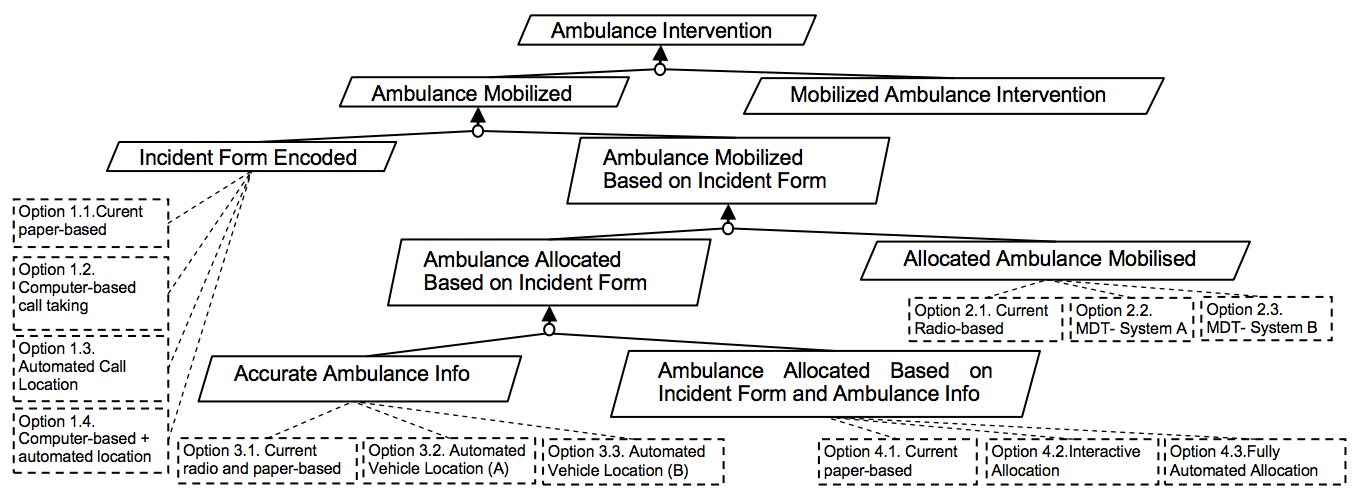
\includegraphics[width=\textwidth]{Chapter-2/figs/KAOS}
    \caption{Partial Goal Model for LAS.}
    \medskip
    \small
    Originally from \cite{heaven11}.
    \label{fig:kaos}
\end{figure}

An example of the KAOS model is shown in \fref{fig:kaos}, depicting a portion of a goal model built for the London Ambulance Service(LAS) case study \cite{finkelstein96}. The top level goal in the figure \textit{``Ambulance Intervention"} has 2 AND dependencies and requires both of them to be satisfied. One of the bottom level goals ``Accurate Ambulance Info" contains 3 OR dependencies and needs only one of them to be satisfied.

Although the KAOS model provides completeness to the requirements documents and traceability between the problem description and solution description, it suffers from few important deficiencies.
\begin{itemize}
    \item KAOS does not model the strategic relationship between the stakeholders.
    \item In situations where the Goals are not quantitative, the relationship between Goals and Agents cannot be categorized using AND and OR dependencies.
\end{itemize}

\subsection{GBRAM}
\label{subsec:bg:gm:gbram}

\begin{figure}[hbtp]
    \centering
    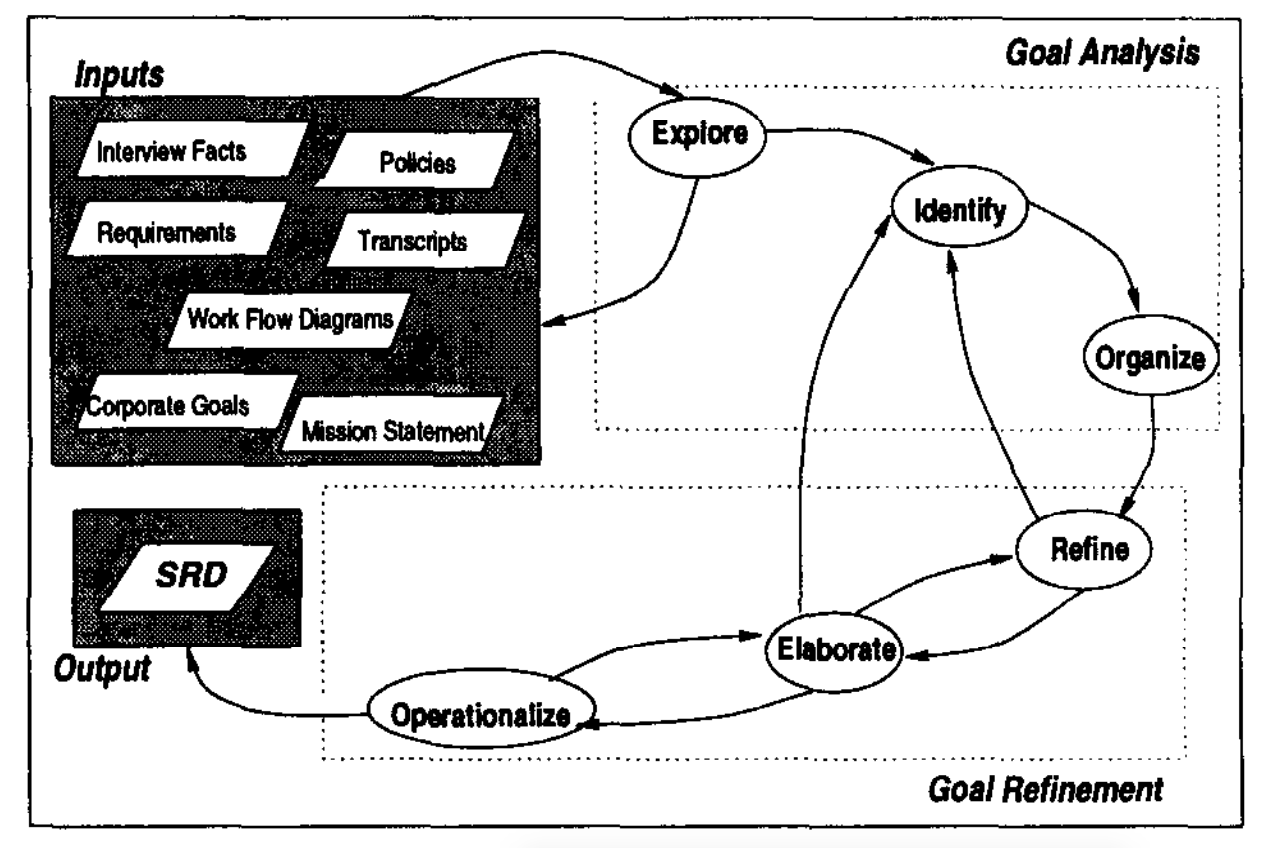
\includegraphics[width=\textwidth]{Chapter-2/figs/GBRAM}
    \caption{Activities in GBRAM.}
    \medskip
    \small
    Originally from \cite{anton98}.
    \label{fig:gbram}
\end{figure}

Anton Et al. proposed GBRAM(\textit{\textbf{G}oal \textbf{B}ased \textbf{R}equirements \textbf{A}nalysis \textbf{M}ethod}) \cite{anton98} which is based on the assumption that goals have not been documented previously and that analysts need to work from different sources of information. \fref{fig:gbram} summarized the two components of GBRAM.\\
\textbf{Goal Analysis:}
\begin{itemize}
    \item \textit{Explore} activities based on available information.
    \item \textit{Identify} activities by extracting goals and the corresponding agents.
    \item \textit{Organize} activities by classifying goals and organizing them based on their dependencies.
\end{itemize}

\textbf{Goal Refinement:}
\begin{enumerate}
    \item \textit{Refine} activities by pruning the set of goals.
    \item \textit{Elaborate} the process of analyzing the goal set by considering possible goal obstacles and constructing scenarios to uncover hidden goals and requirements.
    \item \textit{Operationalize} goals by translating requirements for the final requirements specification.
\end{enumerate}

Like the KAOS model in section \ref{subsec:bg:gm:gbram}, GBRAM suffers from the same problems although the framework introduces the concept of constraints the highlight the relationship between the goals.

\subsection{NFR}
\label{subsec:bg:gm:nfr}

The NFR(\textit{\textbf{N}on-\textbf{F}unctional \textbf{R}equirement}) modeling framework is designed to represent user intentions in technical systems \cite{chung00}. 
An NFR is a type of requirement which is used to evaluate the operation of the system rather than its behaviour based on specific criteria.

The NFR framework decouples the concept  of functionality from other attributes used to justify quality and concerns for productivity, time and cost using a higher level abstraction. Rather than focusing on expressing requirements in the form of descriptive functions, constraints and attributes, NFR uses the concept of \textit{softgoals} which are not satisfied through clear-cut criteria. The framework also incorporates AND and OR decompositions amongst goals and contribution links which represent (partially)positive and (partially) negative contributions to and from softgoals.

The NFR framework addresses the one of the drawbacks of KAOS and GBRAM by using softgoals where dependencies can now be represented as contributions. But the problem of the ``strategic relationship amongst stakeholders" still persists.

\subsection{i*}
\label{subsec:bg:gm:istar}
The i* framework \cite{yu97} is utilizes the key concepts of NFR framework, including softgoals, AND/OR decompositions and contribution links along with goals, resources and tasks. The model addresses the prime drawback of its predecessors by including dependencies between actors(agents).

The i* framework describes dependencies among actors. There are four primary elements to describe the model: \textbf{goal}, \textbf{soft goal}, \textbf{task} and \textbf{resource}. Intentional actor forms the central concept in i*. Organizational actors are viewed as having intentional properties such as goals, beliefs, abilities, and commitments (concept of distributed intentionality). Actors depend on each other for goals to be achieved, tasks to be performed and resources to be generated. By depending on others, an actor may be able to achieve goals that are difficult or impossible to achieve on its own. On the other hand, an actor becomes vulnerable if the actors it depended on did not deliver. Actors are strategic in the sense that they are concerned about opportunities and vulnerabilities, and seek rearrangement of their environments that would better serve their interests by restructuring intentional relationships.

\fref{fig:istar} depicts a sample i* Model for youth counselling. Hexagons represent Tasks; Goals are represented by ellipses; Rectangles represent resources; and Softgoals are represented by the informal shapes.

\begin{figure}[hbtp]
    \centering
    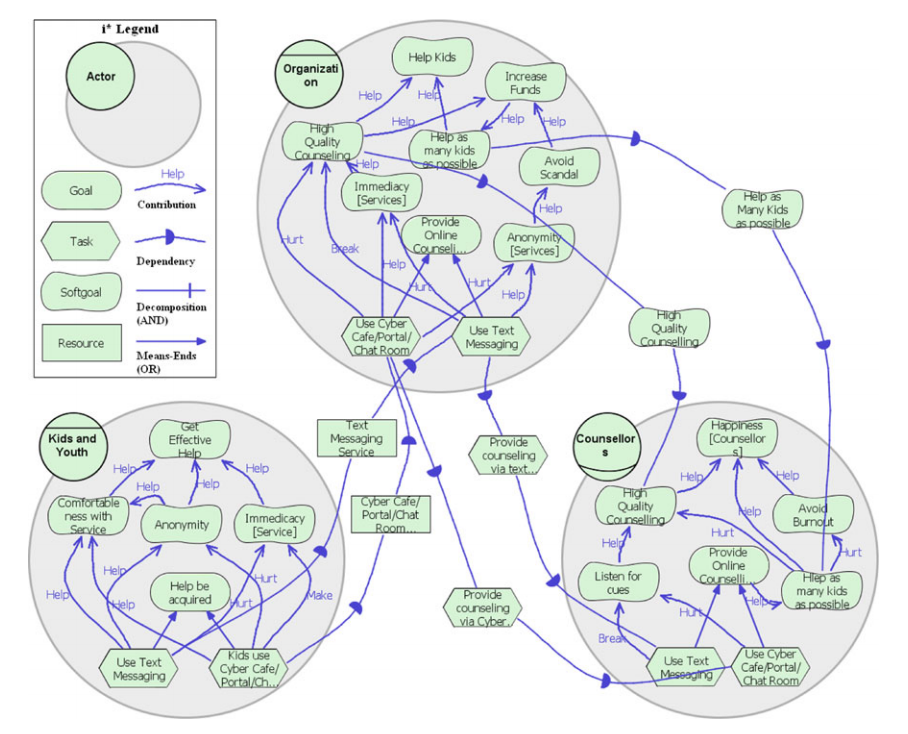
\includegraphics[width=\textwidth]{Chapter-2/figs/istar}
    \caption{Sample i* Model for youth counseling}
    \medskip
    \small
    The legend on the top left indicates the legend for all the components of the i*. Originally from \cite{horkoff12}.
    \label{fig:istar}
\end{figure}


The i* model is very verbose and one of the prime models used in Requirements Engineering. A reduced form the i* model is used in GRL(goal oriented language)\cite{amyot10} and it is also the first stage of TROPOS \cite{giorgini05}, an agent oriented system development methodology.

\subsection{AHP}
\label{subsec:bg:gm:ahp}

The AHP(\textit{\textbf{A}nalytic \textbf{H}ierarchy \textbf{P}rocess}) modelling framework was developed by Thomas Saaty in 1987 for organizing and analyzing complex decisions based on mathematics and psychology \cite{saaty87}. AHP is used extensively in applications like group decision making in fields such as government, business, industry, healthcare, ship building and education \cite{saracoglu13}.

\begin{table}[htbp]
\centering
\begin{tabular}{|c|l|l|}
\hline
\textbf{Scale} & \multicolumn{1}{c|}{\textbf{\begin{tabular}[c]{@{}c@{}}Definition (in terms \\ of Importance)\end{tabular}}} & \multicolumn{1}{c|}{\textbf{Comment}} \\ \hline
1 & Equal & Two activities contribute equally to the objective \\ \hline
2 & Weak & \multirow{2}{*}{\begin{tabular}[c]{@{}l@{}}Experience and judgement slightly favor one \\ activity over another.\end{tabular}} \\ \cline{1-2}
3 & Moderate &  \\ \hline
4 & Moderate plus & \multirow{2}{*}{\begin{tabular}[c]{@{}l@{}}Experience and judgement strongly favor one \\ activity over another.\end{tabular}} \\ \cline{1-2}
5 & Strong &  \\ \hline
6 & Strong plus & \multirow{2}{*}{\begin{tabular}[c]{@{}l@{}}An activity is favored very strongly demonstrated\\ over another.\end{tabular}} \\ \cline{1-2}
7 & Very strong &  \\ \hline
8 & Very very strong & \multirow{2}{*}{\begin{tabular}[c]{@{}l@{}}The evidence favoring one activity over another\\ is of the highest possible order of assumption.\end{tabular}} \\ \cline{1-2}
9 & Extreme &  \\ \hline
\begin{tabular}[c]{@{}c@{}}Reciprocals\\ of above\end{tabular} & Inverse Relation & \begin{tabular}[c]{@{}l@{}}If activity i has one of theabove non-zero numbers\\ assigned to it when compared with activity j, then\\ j has the reciprocal value when compared with i.\end{tabular} \\ \hline
1.1 - 1.9 & Activities are very close & \begin{tabular}[c]{@{}l@{}}Contrasting activities with the size of small numbers\\ with relative importance of activities.\end{tabular} \\ \hline
\end{tabular}
\caption{Scale of priorities used for comparison}
\label{tab:ahp:props}
\end{table}

Saaty described the process of making decisions using AHPs as follows:

\begin{enumerate}
    \item The problem is defined and the kind of knowledge to be sought is determined.
    \item The hierarchy of decisions from the top with the goal of the decision is structured, following which the objectives are structured from a broad perspective though the intermediate levels(factors on which subsequent elements depend) to the lowest level(set of alternatives).
    \item A set of pairwise comparison matrices are constructed. Each element in a higher level is used to compare the elements in the level immediately below with respect to it.
    \item The priorities obtained from the comparisons are used to weight the priorities in the level immediately below. This is repeated for every element. For each element in the level below its weighed values are added and its overall or global priority is obtained. This process of weighing and adding is continued until the final priorities of the alternatives in the bottom most level are obtained.
\end{enumerate}


For the purpose of making comparisons, a scale of numbers that indicates how many times more important or dominant one element is over another element with respect to the criterion or property against which the elements are compared. This scale is highlighted and explained in \tref{tab:ahp:props}.


\section{Multi-Objective Optimization}
\label{sec:bg:moo}

A \textbf{M}ulti-\textbf{O}bjecitve \textbf{O}ptimization(MOO) is a category of mathematical optimization problem which involves more than one objective function to be optimized simultaneously. Mathematically, a MOO can be defined as follows
\begin{equation}
    \begin{aligned}
        & minimize \quad F(x) = (f_1(x), \ldots ,f_m(x))  \\
        & subject\ to \quad x \in \Omega
    \end{aligned}
    \label{eq:MOO}
\end{equation}


where $\Omega$ is the \textit{decision (variable) space}, $R^m$ is the objective space and $F : \Omega \rightarrow R^m$ consists of $m$ real-valued objective functions. If $\Omega$ is a closed and connected region in $R^n$ and all the objectives are continuous of $x$, the problem in \eref{eq:MOO} is categorized as a \textit{Continuous Multi-Objective Optimization Problem}.

Let $a = (a_1, \ldots , a_m), b = (b_1, \ldots , b_m) \in R^m$ be two vectors, then $a$ is said to \textit{dominate} $b$ if $a_i \leq b_i$ for all $i = 1, \ldots, m$, and $a \neq b$.\footnote{This is described for a minimization problem. All the inequalities is reversed to maximize the objective in \cite{miettinen99}. ``Dominate" refers to ``better than".} A point $x^* \in \Omega$ is called \textit{(globally) Pareto optimal} if there is no $x \in \Omega$ such that $F(x)$ dominates $F(x*)$. The set of all the Pareto optimal points is called the \textit{Pareto Set}($PS$). The set of all the Pareto objective vectors is defined as $PF = \{ F(x) \in R^m | x \in PS\}$, is called the \textit{Pareto Front}\cite{miettinen99}.

None of the points on the Pareto front can be said to better than another. This raises a need to find as many Pareto Optimal points as possible. Classically, optimization methods like Simulated Annealing \cite{kirkpatrick83}, Particle Swarm Optimization \cite{kennedy95} and other evolutionary methods\cite{fonseca93} converted the multi-objective optimization problem to a single-objective optimization problem by emphasizing one particular Pareto-optimal solution at a time. Using such methods to find the Pareto Front, the method needs to be applied multiple times with the hope of finding a different point for each simulation run.


\section{Literature Review}
\label{sec:bg:lr}

\subsection{Interactive Analysis}
\label{subsec:bg:lr:interactive}
An interactive goal model analysis was performed by Horkoff Et. al\cite{horkoff12} based on \textit{Forward} and \textit{Backward} Propagation techniques. In forward propagation, the ``satisfaction level" of the goals is propagated onto other goals on the paths of the contributions as defined on the model. On the other hand in the backward propagation method, the model is traced back onto the potential solutions and subsequent goals are checked for their satisfiability by asking questions of the models. While questions are analyzed alternative paths are also considered to satisfy a node. Although this method is highly effective, there is a large amount of human involvement particularly in case of conflicts or cycles in the model which results in constant interruptions. Moreover, the approach also fails to enlist different possible optimum solutions in a single execution run. For a different expected output, the stakeholder has to provide a different input when prompted, thus making the approach cumbersome in case of complex models.

\subsection{Partial Goal Satisfaction Reasoning}
\label{subsec:bg:lr:parGoalSat}
Letier Et. al \cite{letier04} developed an extension of the KAOS  \cite{van09} for reasoning about alternative design choices based on measurable, domain-specific criteria.  In this framework, the degrees of satisfaction for a goal are specified using objective functions defined in terms of quality variables, which are random variables (i.e. functions over probability spaces). For example, they specify the goal Achieve [Ambulance Intervention] from \fref{fig:kaos} in \fref{fig:pgsr}.

\begin{figure}[!hbtp]
    \begin{mdframed}
        \noindent
        \textbf{Goal} Achieve[Ambulance Intervention] 
        
        \noindent
        \textbf{Definition}
        
        \noindent
        For every urgent call reporting an incident, there should be an ambulance at the incident scene within 14 minutes after receiving the first call.
        
        \noindent
        \textbf{Formal Definition}($\forall i:Incident, c:UrgentCall$)
        
        $Reporting(c,i) \implies \diamond_{14mins} (\exists a:Ambulance) Intervention(a,i)$
        
        \noindent
        \textbf{Objective Functions}
        
        $14MinResponseRate = MAX[P(ResponseTime \leq 14 mins)]$
        
        $8MinResponseRate = MAX[P(ResponseTime \leq 8 mins)]$
        
        \noindent
        \textbf{Quality Variable}
        
        $ResponseTime: Incident \rightarrow Time$
        
        \{\textbf{def:} the duration in seconds between the start of the first call reporting the incident and the 
        
        arrival of the first ambulance at the incident scene.\}    
    \end{mdframed}
    
    
    \caption{Quantitative Goal Model Representation for London Ambulance Service}
    \label{fig:pgsr}
\end{figure}



The goal's definition and formal definition define what it means for the goal to be satisfied in an absolute sense; the goal semantic is the set of system behaviours – i.e. sequences of system states – that satisfy the goal's formal definition. The goal objective functions define the measures to be used for assessing partial levels of goal satisfaction. Objective functions are defined in terms of quality variables that correspond to domain phenomena related to the goal's definition. The quality variables associated with a goal can be related to quality variables associated with its sub-goals through domain-specific \textit{refinement equations}. 

This approach exibits the same problem as that of the Interactive model i.e the approach also fails to enlist different possible optimum solutions in a single execution run.


\subsection{Simulation \& Optimization}
\label{subsec:bg:lr:simOpt}

Heaven Et. al \cite{heaven11} overcame these drawbacks by presenting a simulation and optimization framework for evaluating the impact of alternative system decisions on high level goals and for finding optimal decision. The simulation model is then used by a multi-objective optimization component that searches through the design space in order to identify the optimal decision choices. NSGAII\cite{deb02} was their choice of multi-objective optimization algorithm used to search the decision space. Although the approach catered to obtaining a wide range of optimal solutions, it failed when the number of competing requirements exceeded three objectives or for highly constrained models.


% \section{Tables}
% Table \ref{tab:one} is about as simple as they come, to put a formula in a 
% table just use the same methods as putting a formula in a paragraph.  
% Table \ref{tab:two} is a similar table in landscape on a seperate page.  
% %
% \begin{table}
% \caption{Table Example}
% \label{tab:one}
% \begin{center}
% \begin{tabular}{lccl}
% \toprule
% Treatment & No Death & Death & Total\\
% \midrule
% Therapy A & 1295 & 72 & 1367\\
% Therapy B 	& 2294 & 195 & 2489\\
% \midrule
% Total & 3589 & 267 & 3856\\
% \bottomrule
% \end{tabular}
% \end{center}
% \end{table}

% \paragraph{Filler Text} \lipsum[1-2]
% \newgeometry{margin=1in,lmargin=1.25in,footskip=\chapterfootskip, includehead, includefoot}
% %\thispagestyle{lscape}
% %\pagestyle{lscape}
% \thispagestyle{lscapedplain}
% \begin{landscape}
% \begin{table}
% \caption{Landscape Table Example}
% \label{tab:two}
% \begin{center}
% \begin{tabular}{lcccccccccl}
% \toprule
% Patient & A & B & C & D & E & F & G & H &I & Total \\
% \midrule
% John & 1 & 2 & 3 & 4 & 5 & 6 & 7 & 8 & 9 & 45 \\
% Amy & 1 & 2 & 3 & 4 & 5 & 6 & 7 & 8 & 9 & 45 \\
% Jim & 1 & 2 & 3 & 4 & 5 & 6 & 7 & 8 & 9 & 45 \\
% Jason & 1 & 2 & 3 & 4 & 5 & 6 & 7 & 8 & 9 & 45 \\
% Sandy & 1 & 2 & 3 & 4 & 5 & 6 & 7 & 8 & 9 & 45 \\
% Icem & 1 & 2 & 3 & 4 & 5 & 6 & 7 & 8 & 9 & 45 \\
% \midrule
% Total & 6 & 12 & 18 & 24 & 30 & 36 & 42 & 48 & 54 & 270\\
% \bottomrule
% \end{tabular}
% \end{center}
% \end{table}
% \end{landscape}
% %\newgeometry{margin=1in,lmargin=1.25in,footskip=\chapterfootskip, includehead, includefoot,landscape=false}
% \restoregeometry
% \pagestyle{fancy}
% \thispagestyle{fancy}
% \newgeometry{margin=1in,lmargin=1.25in,footskip=\chapterfootskip, includehead, includefoot}


% \section{Figures}

% The easiest way to insert a picture is to have that picture in pdf format.  
% \fref{fig:hist1} and \fref{fig:hist2} are two figures typeset normally.
% ETD guidelines allow the use of landscape pages in the electronic 
% submission.  To rotate a page, do NOT use the \texttt{lscape} environment. Instead, use the \texttt{pdflscape} package, for compatibility with PDFlatex.
% Please note, if you are preparing a document for binding, consider
% giving the \texttt{hardcopy} option in the \verb|\documentclass|
% declaration.  This will place the page number at the normal location,
% which is where it should be for printing and binding.
% %
% \begin{figure}[hbtp]
% \centering
% 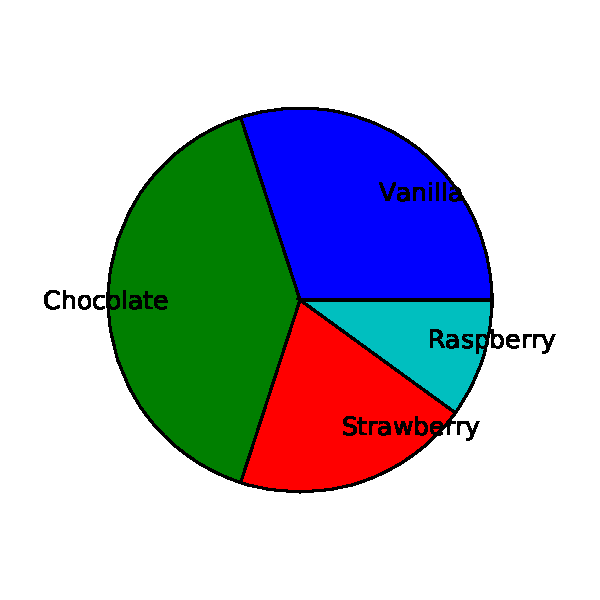
\includegraphics[width=0.6\textwidth]{Chapter-2/figs/pie}
% \caption{Here is a sample figure}
% \label{fig:hist1}
% \end{figure}

% For an example of a figure with a really long caption, see Fig.~\ref{fig:longcap}
% \begin{figure}[hbtp]
% \centering
% \calculategraphicstargetheight{11}
% 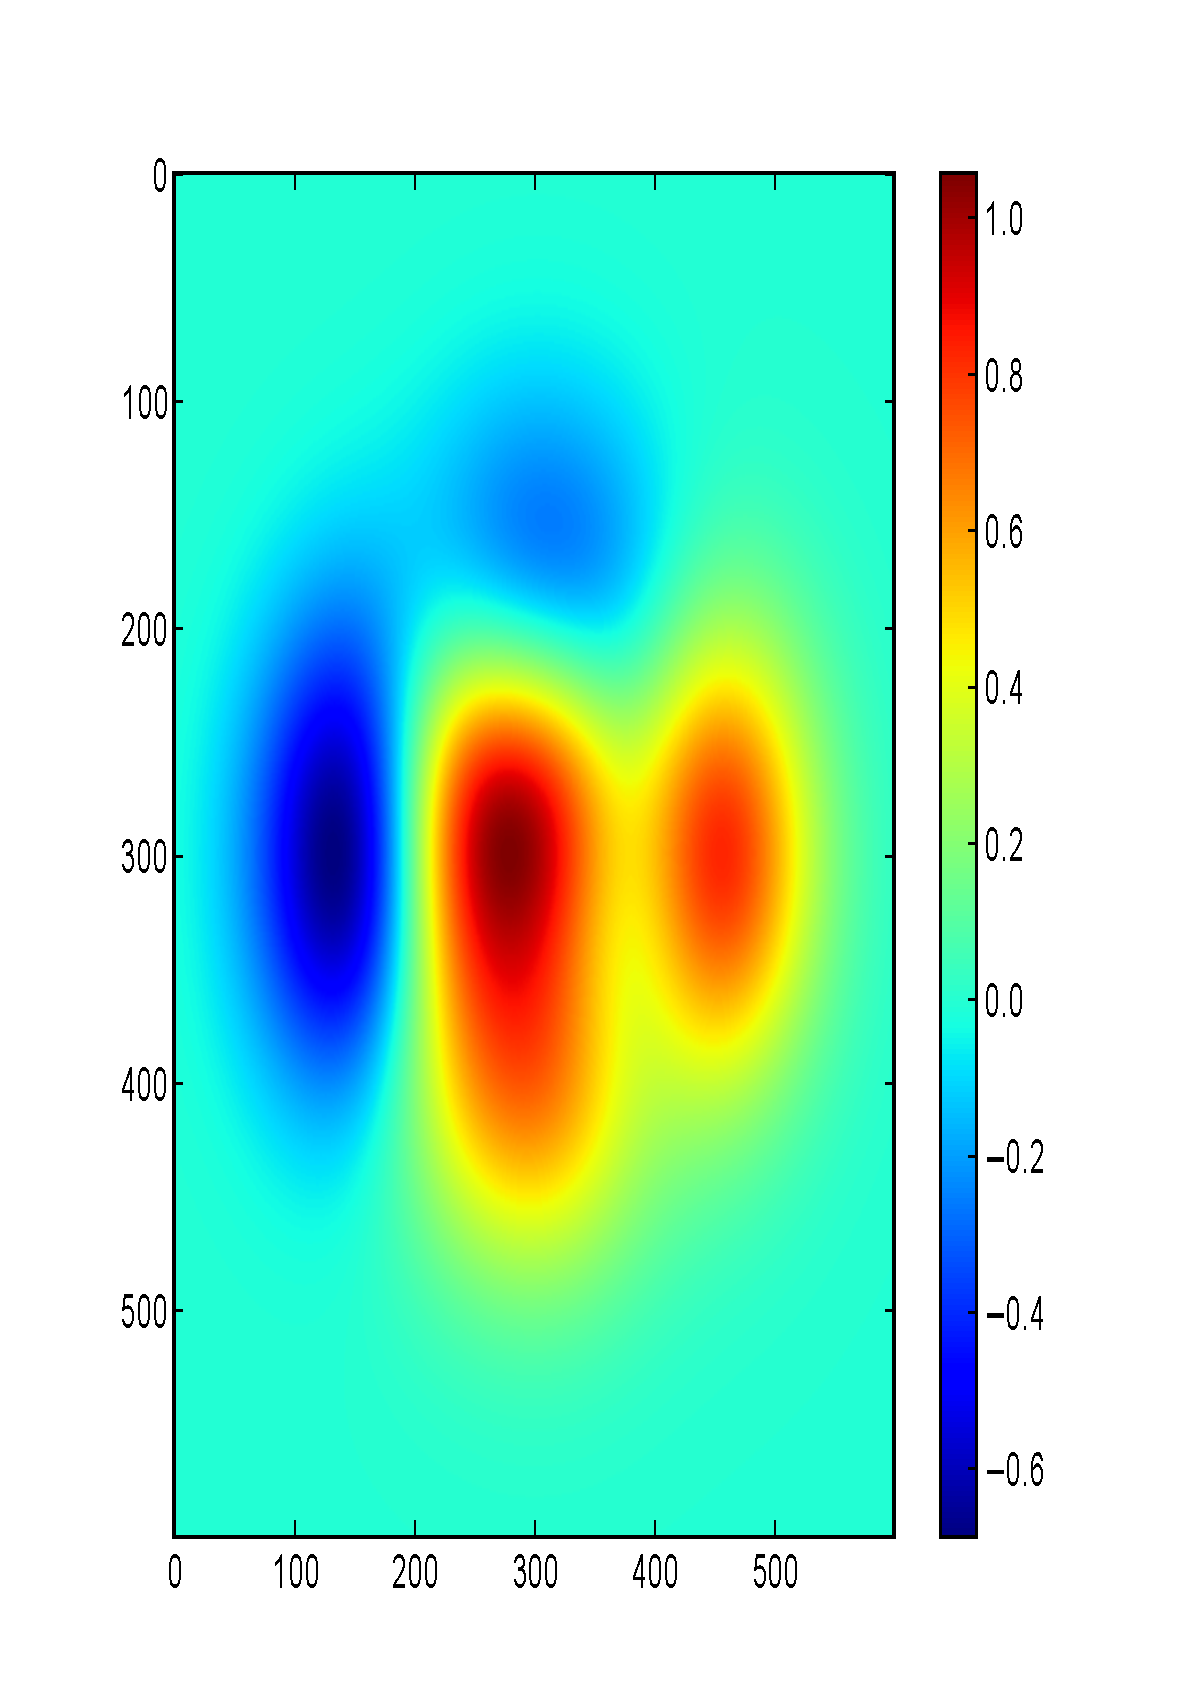
\includegraphics[height=\graphht]{Chapter-2/figs/color_stretched}
% \caption{Here is a HUGE sample figure with a HUGE caption. Our goal is to make a caption that is so long that the caption spills into the lower margin, leading to an ETD error. The way to solve this problem in a systematic way is to calculate how many lines of text the caption will use, then adjust the size of the image, such that it leaves just enough space for your huge caption. How I am solving this problem is by providing a new variable called graphht that stores how tall the image should be. Then, to calculate how tall to make the figure, you use the new function that I am providing called calculategraphicstargetheight. This function has one argument. The argument of the function is how many lines of text you estimate that the caption occupies. You can always run your tex once, measure this number, and type it into the argument for the function. What the function will do (it is defined in the preamble) is take into account the size you give it, the spacing of the chapter and the footer at the bottom, 
% and then calculate the total vertical space available. Thus, this function should be used for images that are taller than they are wide.}
% \label{fig:longcap}
% \end{figure}
% %
% \begin{figure}[hbtp]
% \centering
% 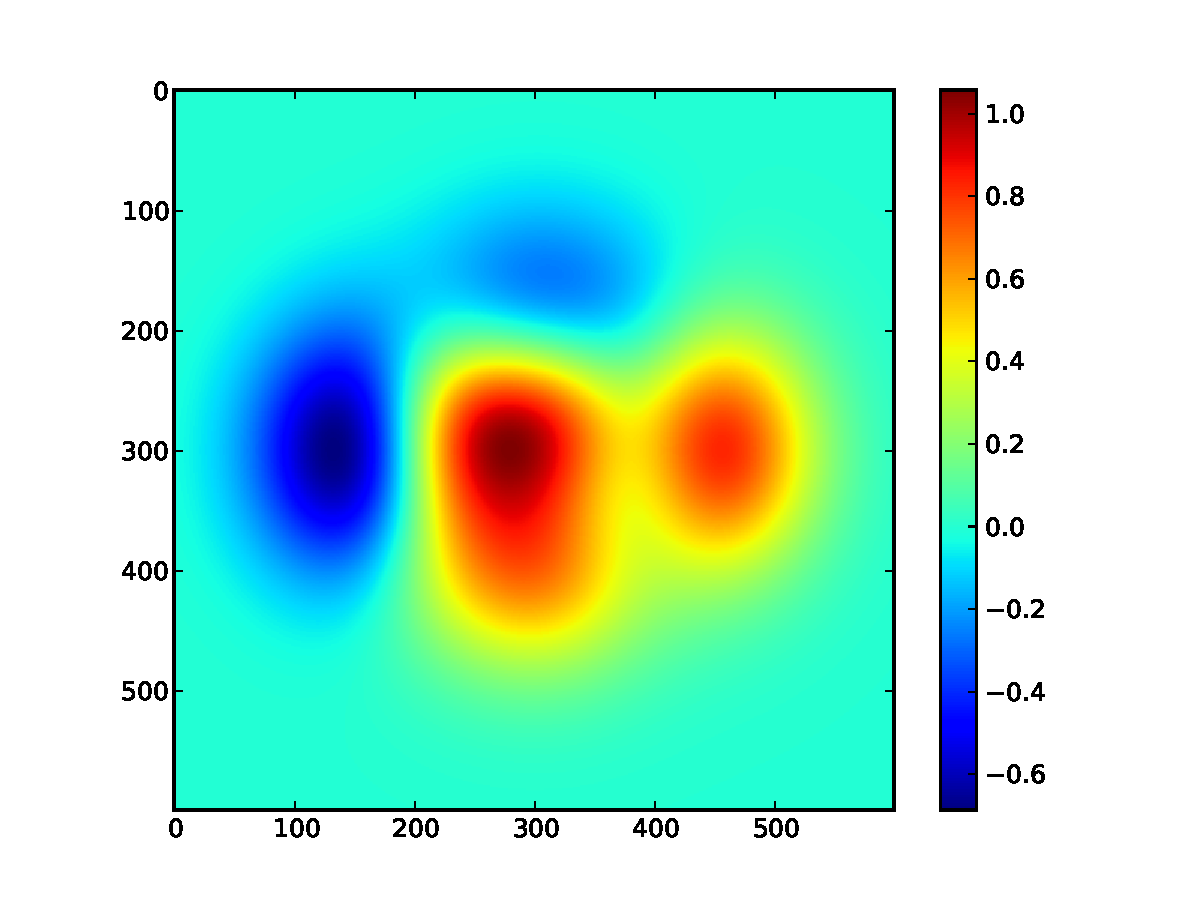
\includegraphics[width=0.6\textwidth]{Chapter-2/figs/color}
% \caption{Here is a sample figure}
% \label{fig:hist2}
% \end{figure}
% %
% \begin{figure}[hbtp]
% \centering
% \subfloat[]{
% 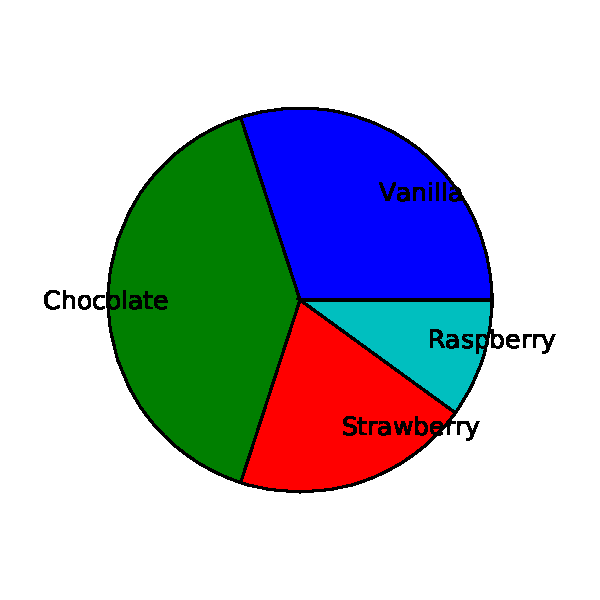
\includegraphics[width=0.4\textwidth]{Chapter-2/figs/pie}
% }
% \subfloat[]{
% 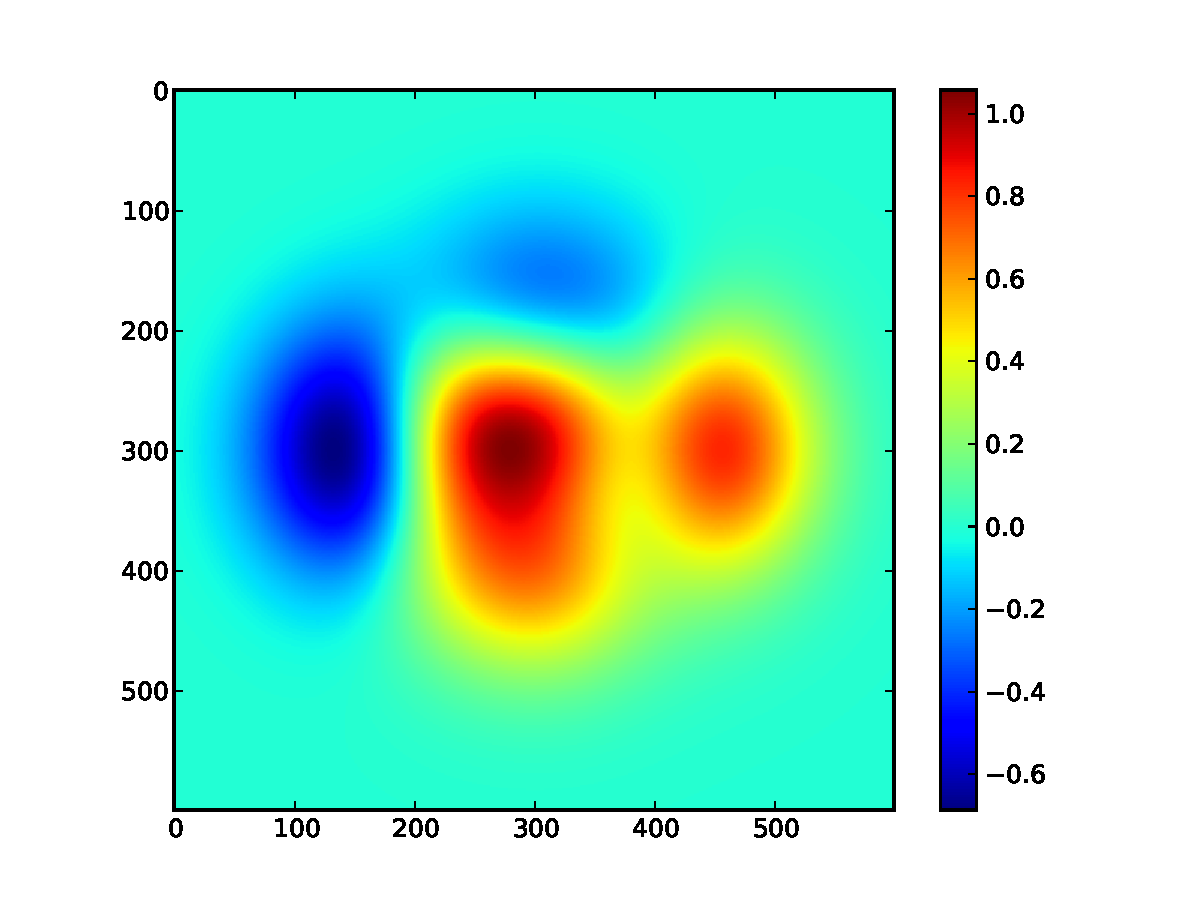
\includegraphics[width=0.4\textwidth]{Chapter-2/figs/color}
% }
% \caption{Here are two floating subfigures}
% \label{fig:subfigures}
% \end{figure}


% \paragraph{Filler Text} \lipsum[12-15]

% \newgeometry{margin=1in,lmargin=1.25in,footskip=\chapterfootskip, includehead, includefoot}
% %\thispagestyle{lscaped}
% %\pagestyle{lscaped}
% \thispagestyle{lscapedplain}
% \begin{landscape}
% \begin{figure}
% \centering
% 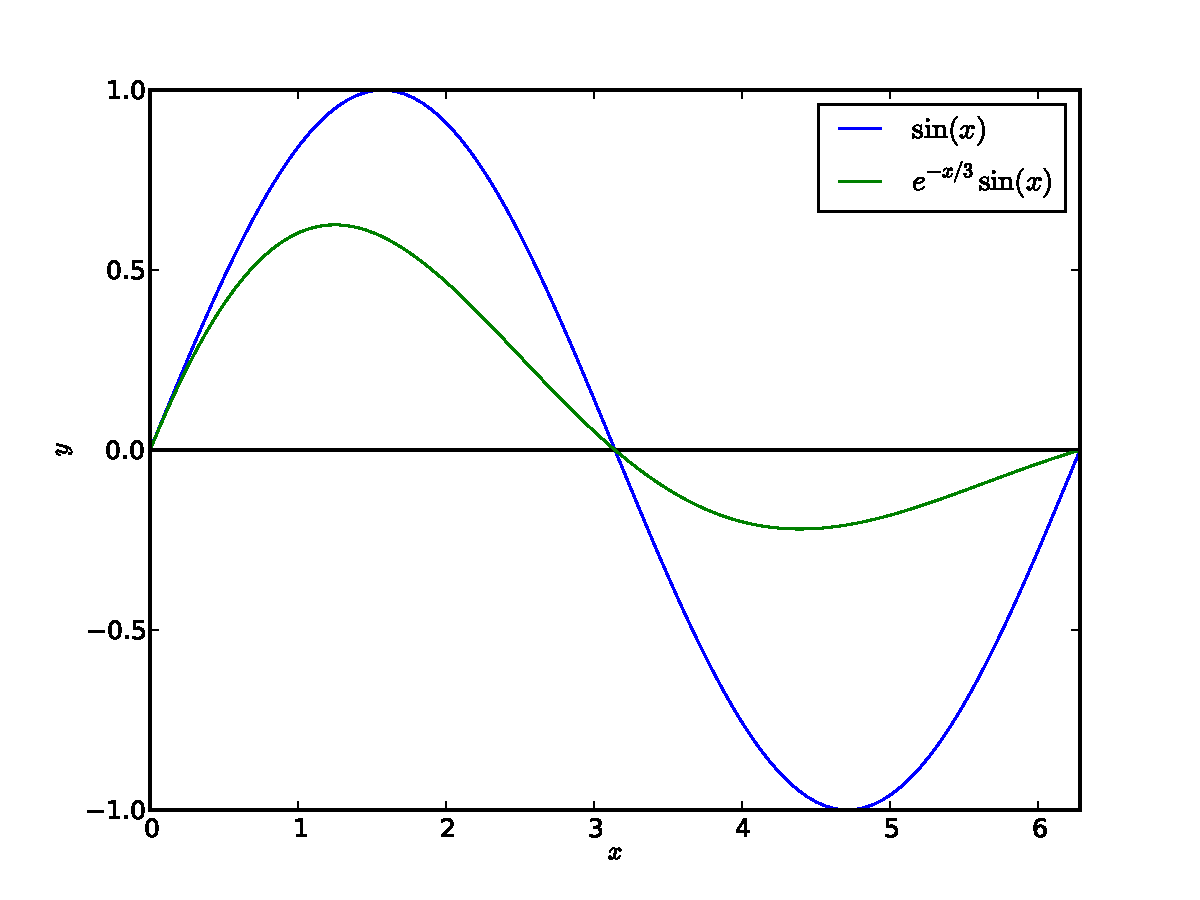
\includegraphics[width=\textwidth]{Chapter-2/figs/sine}
% %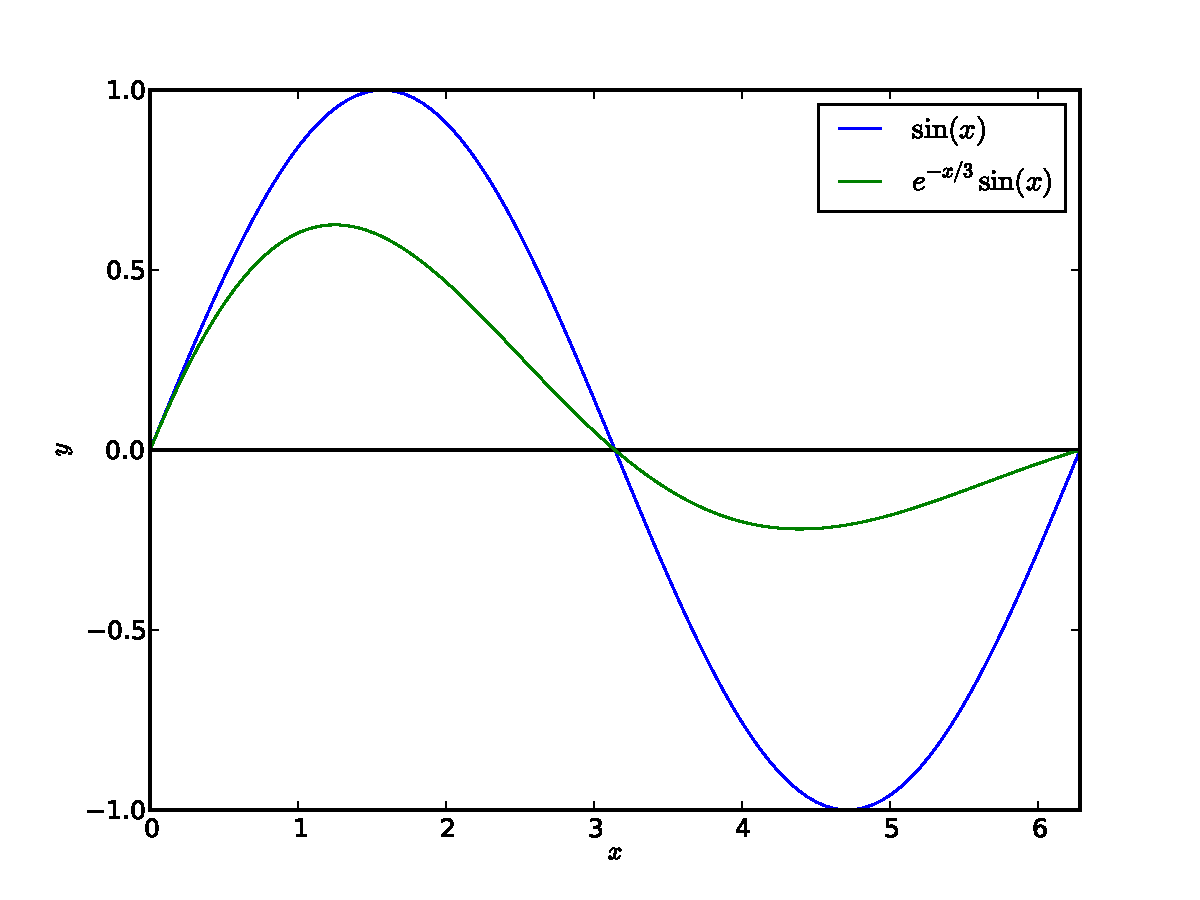
\includegraphics[height=\textwidth]{Chapter-2/figs/sine}
% \caption{This figure has been turned sideways.  With large figures, 
%          the author must ensure that there are at least two double spaces
%          between the caption and the page number.}
% \label{fig:hist}
% \end{figure}
% \end{landscape}
% %\newgeometry{margin=1in,lmargin=1.25in,footskip=\chapterfootskip, includehead, includefoot,landscape=false}
% \restoregeometry
% \pagestyle{fancy}
% \thispagestyle{fancy}
% \newgeometry{margin=1in,lmargin=1.25in,footskip=\chapterfootskip, includehead, includefoot}


% \section{Matrices}
% Let's look at a simple example of a matrix:
% \[ \left( \begin{array}{ccc}
% a & b & c \\
% d & e & f \\
% g & h & i \end{array} \right)\] 
% %
% You may prefer to write it this way:
% \[ \left[\begin{array} {cccccc}
% 1 & 0 & 0 & 0 & 0 & 0 \\
% 0 & 1 & 0 & 0 & 0 & 0 \\
% 0 & 0 & 1 & 0 & 0 & 0 \\
% 0 & 0 & 0 & 1 & 0 & 0 \\
% 0 & 0 & 0 & 0 & 1 & 0 \\
% 0 & 0 & 0 & 0 & 0 & 1 \\
% \end{array} \right] \]

\chapter{LOREM IPSUM}

\section*{A First Section}

\paragraph{Filler Text} \lipsum[1-6]
%
\begin{figure}[t]
  \centering
  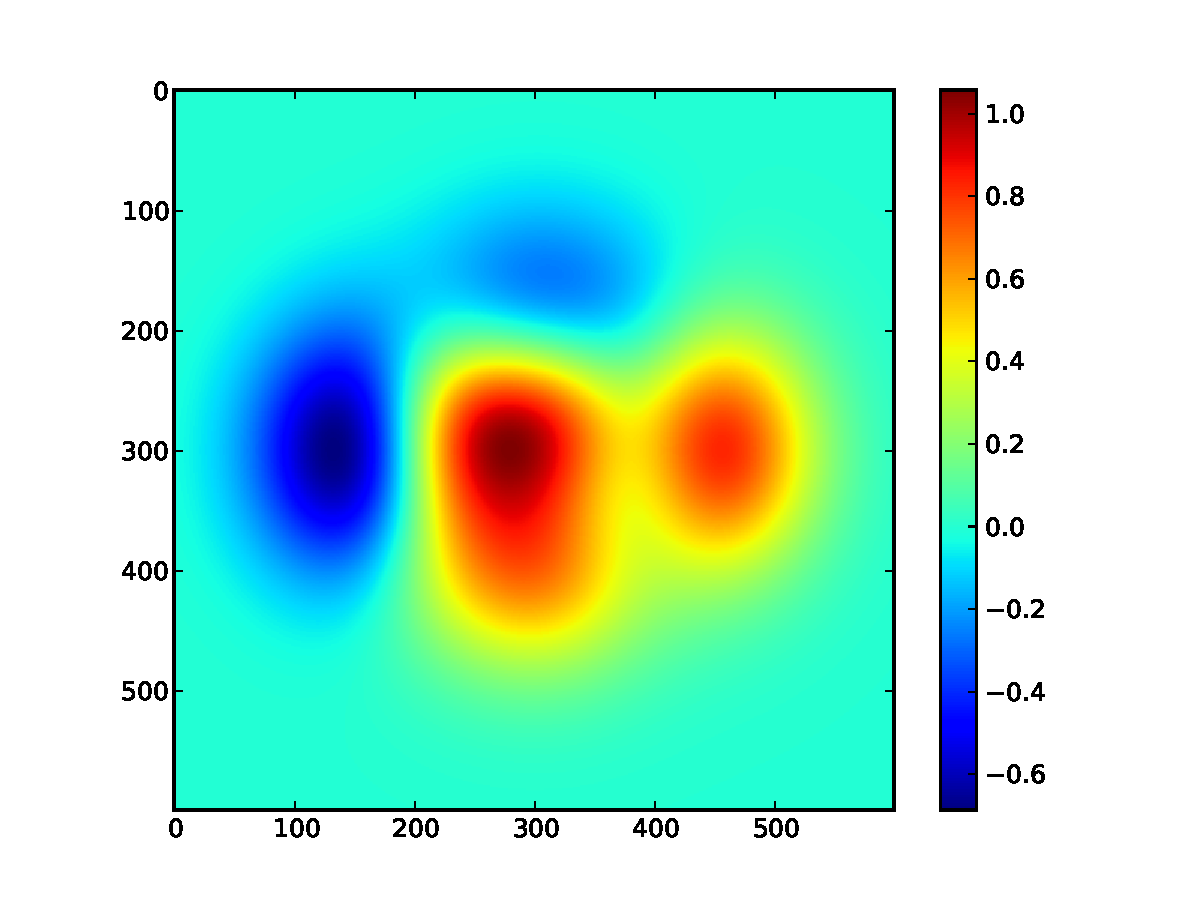
\includegraphics[width=0.6\textwidth]{Chapter-2/figs/color}
  \caption{A figure at the top of the page.}
  \label{fig:ch3.1}
\end{figure}
%
\lipsum[7-13]
%
\begin{figure}[!h]
  \centering
  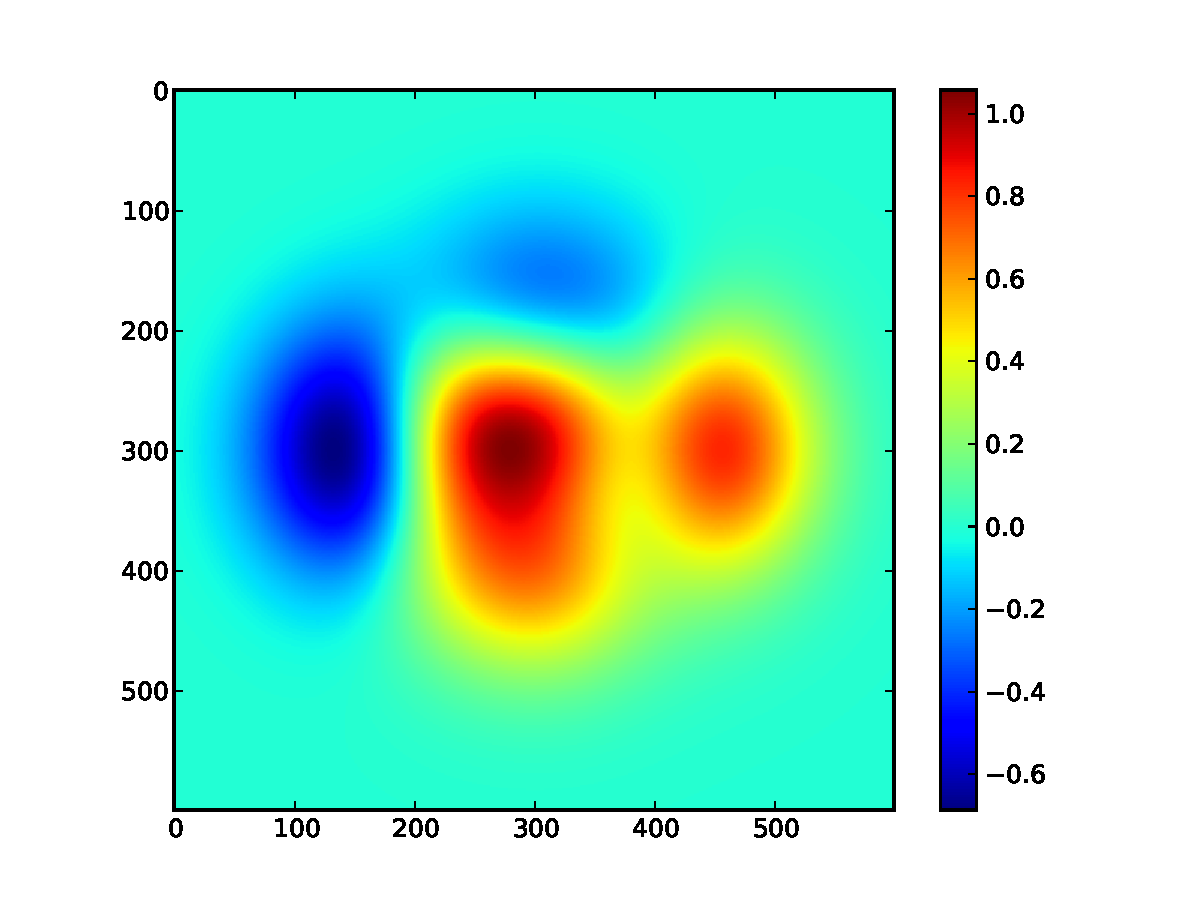
\includegraphics[width=0.6\textwidth]{Chapter-2/figs/color}
  \caption{A figure in the middle of text.}
  \label{fig:ch3.2}
\end{figure}
%
\begin{figure}[!b]
  \centering
  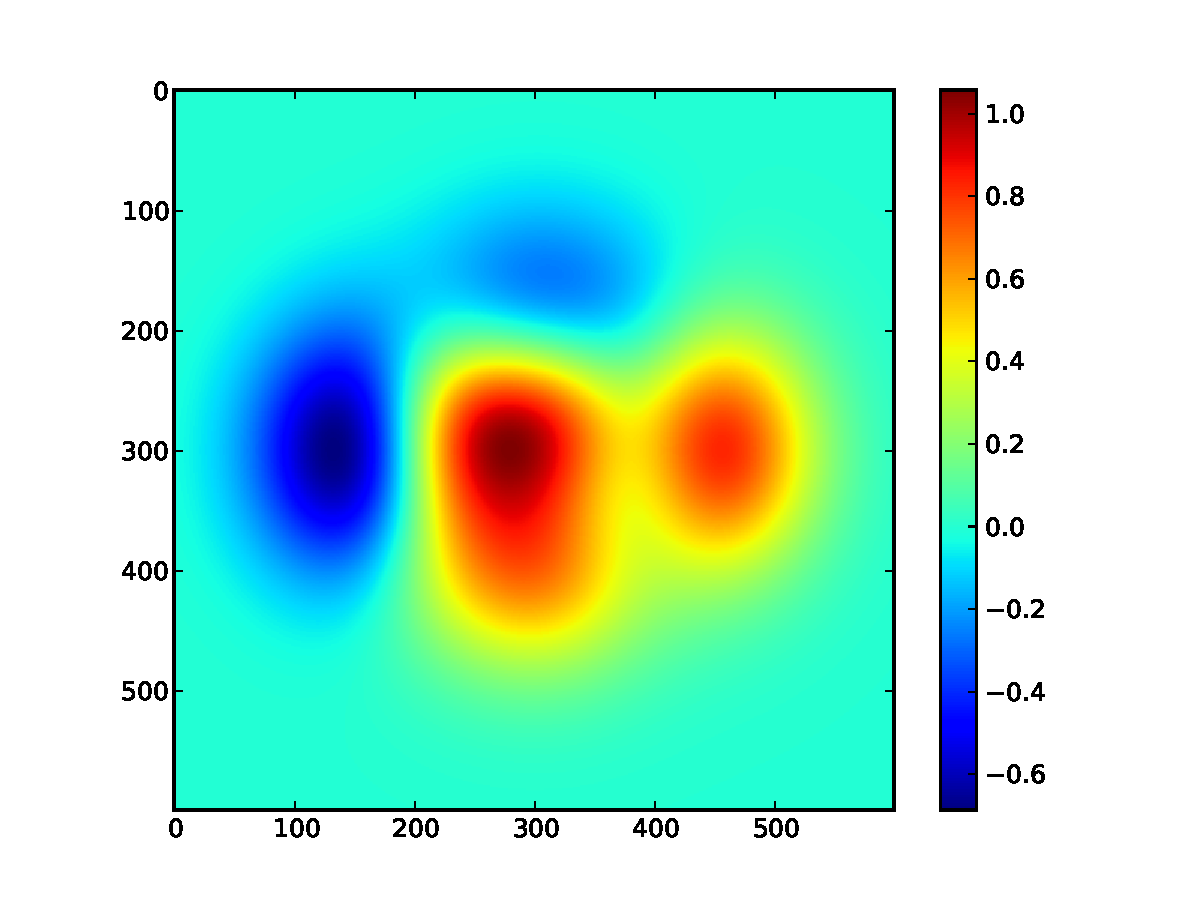
\includegraphics[width=0.6\textwidth]{Chapter-2/figs/color}
  \caption{A figure at the bottom of the page.}
  \label{fig:ch3.3}
\end{figure}
%
\lipsum[14-20]

%\chapter{Search Algorithm}
\label{chap:sa}

In chapter \ref{chap:model} we defined the internal space of our models. We now look to optimize it. Differential Evolution, a multi-objective optimization algorithm is used to optimize the decision space as per the stakeholders requirements(objectives) and post which a bayesian selection algorithm is used to rank the design decisions of the model according to how well they satisfy the objectives.

\section{Differential Evolution}
\label{sec:sa:de}
\textit{Meta-heuristics} are higher-level procedures or heuristics designed to find, generate, or select a heuristic that may provide a sufficiently good solution to an optimization problem, especially with incomplete or imperfect information or limited computation capacity. Meta-heuristics sample a set of solutions which is too large to be completely sampled. Meta-heuristics may make few assumptions about the optimization problem being solved, and so they may be usable for a variety of problems. Meta-heuristics are also based of Monte Carlo algorithms. A \textit{Monte Carlo} algorithm randomly samples the space of possible controllable model states. A \textit{Metropolis} Monte Carlo algorithm \cite{metropolis53} creates new states by small mutations to the current state. If a new state is ``better" (as assessed through the domination of the decisions with respect to the objectives of the model), it replaces the current state and us used for future mutations.

\textbf{D}ifferential \textbf{E}volution(DE) is a meta-heuristic evolutionary computation method that can find the Pareto Front of the multi-objective optimization problem without converting it into a single-objective optimization one. DE optimizes a problem by iteratively trying to improve a candidate solution with regard to a specific measure(s) of quality. DE does not make any assumptions on the nature of the optimization problem and does not require the problem to be continuous or differentiable.


\begin{algorithm}[!hbtp]
\caption{Differential Evolution}
\label{algo:DE}
\begin{algorithmic}[1]
\State Generate randomly an initial population($P$) of solutions where each solution $x \in R^n$.
\State Calculate the fitness of the initial population.
\Repeat
    \For{each point $p \in P$}
        \State Pick 3 other points $a$, $b$ \& $c$ from $P$ where $a,b,c \neq p$
        \State Pick a random index $R \in {1, \ldots, n}$
        \For{$i \in n$}
            \State $r_i \in U(0,1)$
            \If{$r_i \le CR$ or $i = R$} 
                \State $y_i = a_i + F * x_i *  (b_i - c_i)$
            \Else
                \State $y_i = x_i$
            \EndIf
        \EndFor
        \If{$f(y) < f(x)$}
            \State replace $x$ with $y$ in $P$
        \EndIf
    \EndFor
\Until {Stop condition is satisfied}
\State $P$ now represents the Pareto Front
\end{algorithmic}
\end{algorithm}

Algorithm \ref{algo:DE} describes the generic approach for the Differential Evolution algorithm. The parameter $F \in [0,2]$ on line 10 represents \textit{differential weight} and $CR \in [0,1]$ on line 9 represents the crossover rate. Both these parameters are chosen based on the problem and requires engineering judgement or tuning to be correctly chosen.

For our models there are a few changes we incorporate that is different to the classical differential evolution method. We change the random generation by introducing the structure of the model while generation and we augment the mutation operation in line 10 to support binary variables.

\subsection{Generation}
\label{subsec:sa:de:gen}

The classical Differential Evolution algorithm uses random generation for the initial population i.e the decisions are randomly sampled across the entire model decision space. We propose a modified method that utilizes the structure of the model for sampling the initial population.

\begin{algorithm}[!hbtp]
\caption{Generation}
\label{algo:DE:gen}
\begin{algorithmic}[1]
    \Procedure{generate}{$tree$, $node$, $value$}
        \State $kids = \bm{GET\_KIDS}(tree, node)$
        \If{$kids == null$}
            \State \Return $\{\bm{ID}(node)\ :\ value\}$
        \EndIf
        \State $decisions = \{ \ \}$
        \State $e\_type = kids[0].edge$
        \State $kids = \bm{SHUFFLE}(kids)$
        \If {($e\_type == ``and" \ \&\&\ value==t) \quad||\quad (e\_type == ``or" \ \&\&\  value==f$)}
            \For{each $kid$ in $kids$}
                \State $\bm{UPDATE}(decisions,\ \bm{GENERATE}(tree,\ kid,\ value))$
            \EndFor
        \Else
            \State $first, rest$ = $\bm{LOO}(kids)$
            \State $\bm{UPDATE}(decisions,\ \bm{GENERATE}(tree,\ kid,\ value))$
            \For{each $kid$ in $rest$}
                \State $\bm{UPDATE}(decisions,\ \bm{GENERATE}(tree,\ kid,\ \bm{choice}(t, f)))$
            \EndFor
        \EndIf
    \EndProcedure
\end{algorithmic}
\end{algorithm}

The modified \textbf{generation} algorithm is defined in Algorithm \ref{algo:DE:gen}. The function is called by passing the model(represented as tree), the root node(represented as node) and the expected value($t$ represents satisfied and $f$ represents unsatisfied). On line 2 the incoming nodes(kids) of the node is retrieved and if there are no incoming nodes a map containing with the node id as the key and the expected value is returned. On lines 6 an empty dictionary is declared and on line 7 edge type of the incoming children are retrieved. The children are randomly shuffled in line 8. On lines 9-13, if the incoming edge is of type AND and the expected value is satisfied or if the incoming edge is of type OR and the expected values is unsatisfied, each incoming node is recursively called with the expected value. This is because for a node with AND edge to be satisfied, all the incoming nodes needs to be satisfied and similarly for a node with an OR edge to be unsatisfied all the incoming nodes needs to be unsatisfied. In the alternate case on lines 13 to 19 one of the incoming nodes($first$) is satisfied for an OR edge and one the incoming nodes is unsatisfied for an AND edge. For all the remaining nodes($rest$), each node is recursively called with a random expected value.

\subsection{Mutation \& Crossover}
\label{subsec:sa:de:mut}

Storn classically proposed using differential mutation and crossover strategy \cite{storn96} but this can only be applied only to continuous decision spaces(As shown on line 10 of Algorithm \ref{algo:DE}). Since the goal models we deal with are binary in nature, we take an alternate method of mutation as shown in \cite{falco07}. The method is defined in \eref{eq:DE:binary}.

\begin{equation}
    \begin{aligned}
        & X_{new} = X_1 \lor (FV \land (X_2 \oplus X_3))\\
        & FV = \{0, 1\}^n \quad where\ n = length(X_{1}) \\
        & FV_i = 1,\quad if\ Random() < F \\
        & \quad \ \ \ \, = 0,\quad otherwise 
    \end{aligned}
    \label{eq:DE:binary}
\end{equation}

Three decision vectors are selected at random. In the vector 1 represents a satisfied and 0 represents an unsatisfied decision. FV is a random vector whose length is equal to the number of decisions. $\lor$ represents a logical OR operator, $\land$ represents a logical AND operator and $\oplus$ represents a logical XOR operator.

\bigskip

\noindent
In terms of the goal of this thesis, exploring the decision subset selection is an essential feature.

\begin{itemize}
    \item Prior to removing unimportant decisions, we rank them with respect to their effectiveness in contribution towards the objectives.
    \item After removal of the non-essential decisions we see the contribution of the reduced model towards the objectives and the savings in the cost. 
\end{itemize}

\section{Support Based Bayesian Ranking}
\label{sec:sa:bayes}

Each decision in the model contributes towards the objectives. Some decisions contribute more than others and if such decisions are identified, the complexity of the model can be reduced. Menzies Et. Al. proposed a support based bayesian ranking algorithm \cite{menzies07} that ranks the decisions using a Simulated Annealer \cite{kirkpatrick83}. We adapt this approach but replace the simulated annealer with differential evolution and also introduce non-dominated sorting.

\begin{figure}
    \begin{mdframed}[backgroundcolor=white]
        \begin{center}
            {\bf Non Dominated Sorting}\\
        \end{center}
        Non Dominated Sorting was a fast objective sorting approach was developed by Srinivas and Deb \cite{srinivas94}. The algorithm is described as follows.
        \bigskip
        \begin{compactitem}
            \item \boldm{P} is a set of points to be sorted and \boldm{k} top points have to be retrieved.
            \item For each individual \boldm{p} in the set \boldm{P}.
            \begin{compactitem}
                \item Initialize \boldm{S_p} = []. This set would contain all the points dominated by p.
                \item Initialize \boldm{n_p} = 0. This would be the number of points that dominate p.
                \item For each point \boldm{q} in \boldm{P}
                \begin{compactitem}
                    \item If \boldm{p} dominates \boldm{q} then
                        \begin{compactitem}
                            \item Add q to set 
                        \end{compactitem}
                    \item Else If \boldm{q} dominates \boldm{p} then
                        \begin{compactitem}
                            \item Increment \boldm{n_p} by 1.
                        \end{compactitem}
                \end{compactitem}
            \end{compactitem}
            \item If \boldm{n_p} = 0 then
                \begin{compactitem}
                    \item Set rank of \boldm{p} to 1.
                    \item Update the first front set by adding \boldm{p} to first front(\boldm{F_1}).
                \end{compactitem}
            \item Initialize front counter to 1; i.e \boldm{i} = 1.
            \item While \boldm{F_i} is not empty
                \begin{compactitem}
                    \item Initialize \boldm{Q} = []; i.e Set of all points in $(\bm{i} + 1)^{th}$ front.
                    \item For each individual \boldm{p} in \boldm{F_i}.
                    \begin{compactitem}
                        \item For each individual \boldm{q} in \boldm{S_p}
                        \begin{compactitem}
                            \item Decrement \boldm{n_q} by 1.
                            \item If \boldm{n_q} = 0 then
                            \begin{compactitem}
                                \item Set rank of \boldm{q} to (\boldm{i} + 1).
                                \item Update Q with \boldm{q}.
                            \end{compactitem}
                        \end{compactitem}
                    \end{compactitem}
                    \item Increment the front counter \boldm{i} by 1.
                    \item Set \boldm{Q} as the next front; i.e \boldm{F_i} = \boldm{Q}.
                \end{compactitem}
            \item Return the top \boldm{k} points from the top fronts.
        \end{compactitem}
        \bigskip
        In the algorithm the term \bit{dominate} refers to Pareto Dominance \cite{deb01} and is mathematically defined in section \ref{sec:bg:moo}.
    \end{mdframed}
    \caption{Non Dominated Sorting}
    \label{fig:non_dom}
\end{figure}

We first rank the decisions using \boldm{K} runs of the differential evolution algorithm. The \boldm{K} runs are divided based on Non Dominated Sorting as described in \fref{fig:non_dom} into:

\begin{itemize}
    \item \textit{Best} : Points associated with the top \boldm{BEST}\% points.
    \item \textit{Rest} : Points that are not included in best.
\end{itemize}

The algorithm then computes the probability that a decision is found in \textit{best} using Bayes' Theorem. Informally, the theorem says that $posterior = prior * likelihood$ ;i.e. what we'll believe next($posterior$) comes from how the $likelihood$ effects with our $prior$ beliefs. More formally:

\begin{equation}
    P(H|E) = P(E|H) * \dfrac{P(H)}{P(E)}
    \label{eq:bayes}
\end{equation}

i.e using evidence $E$ and a prior probability $P(H)$ for hypothesis $H \in \{best, rest\}$. The theorem calculates the posterior probability $P(H|E)$. Simple Bayes classifiers are often called ``naive" since they assume independence of each feature. While this assumption simplifies the implementation(frequency counts are required only for each decision), it is possible that correlated events are missed by this naive approach. Domingos and Pazzani show theoretically that the independence assumption is a problem in a vanishingly small percent of cases \cite{domingos97}. This explains the repeated empirical result that, on average, seemingly naive Bayes classifiers perform as well as other seemingly more sophisticated schemes.

When applying the theorem, \textit{likelihoods} are computed from observed frequencies, then normalized to create probabilities (this normalization cancels out $P(E)$ in \eref{eq:bayes}, so it need not be computed). For example after K = 10,000 runs divide into 1,000 lowest 10\% \textit{best} solutions and 9,000 \textit{rest}, the decision $2Tier = satisfied$ from \fref{fig:ahp} might appear 10 times in the \textit{best} solutions, but only 5 times in the rest. This can be formulated as follows:

\begin{equation}
    \begin{aligned}
        E &\quad =\quad (2Tier == satisfied) \\
        P(best) &\quad =\quad 1000 / 10000 = 0.1 \\
        P(rest) &\quad =\quad 1000 / 10000 = 0.1 \\
        freq(E|best) &\quad =\quad 10/1000 = 0.01 \\
        freq(E|rest) &\quad =\quad 5/9000 = 0.00056 \\
        like(best|E) &\quad =\quad freq(E|best) * P(best) = 0.001\\
        like(rest|E) &\quad =\quad freq(E|rest) * P(rest) = 0.000504\\
        P(best|E) &\quad =\quad \dfrac{like(best|E)}{like(best|E) + like(rest|E)}
    \end{aligned}
    \label{eq:posterior}
\end{equation}

Clark found that \eref{eq:posterior} is a poor ranking heuristic since it is distracted by low frequency evidence \cite{clark05}. For example, note how the probability of $E$ belonging to the best class is moderately high even though its support is very low; i.e $P(best|E) = 0.66$ but $freq(E|best) = 0.01$.

To avoid such unreliable low frequency evidence, \eref{eq:posterior} is augmented with a support term. Support should \textit{increase} as the frequency of a range \textit{increases},i.e $like(best|x)$ is a valid support measure. STAR1 algorithm thus ranks the decisions using \eref{eq:star1}.

\begin{equation}
    \begin{aligned}
        P(best|E) * support(best|E) &\quad = \quad \dfrac{like(best|x)^2}{like(best|x) + like(rest|x)}
    \end{aligned}
    \label{eq:star1}
\end{equation}


\section{The STAR1 Algorithm}
\label{sec:sa:star1}

STAR1 was a framework proposed by Menzies Et. Al \cite{menzies07} that utilized an optimizer and a ranker to rank the decisions. We include Differential Evolution as an optimizer and the Bayesian ranker from Section \ref{sec:sa:bayes} as the ranker for the framework. The STAR1 runs in six phases. With respect to standard machine learning theory, step 1 generates a training set; sets 2 and 3 performs some generalization; step 4 tests the learned theory on the data; and step 5 reports our learning.

\begin{itemize}
    \item \bit{SAMPLE}: To sample the decisions form the models, STAR1 runs the Differential Evolution algorithm $\bm{K_1}$ times.
    \item \bit{CLASSIFY}: The outcomes of the runs are then ranked into those seen in $\bm{BEST}$\% as \textit{best} and the remaining into \textit{rest}.
    \item \bit{RANK}: The decisions along with their optimal values are then ranked using Non Dominated Sorting as depicted in \fref{fig:non_dom} in the decreasing order by their $probability\ *\ support$ \eref{eq:star1} of appearing in the \textit{best} outcomes.
    \item \bit{PRUNE}: The algorithm then runs $\bm{K_2}$ experiments with the models where the top ranked decisions 1 \ldots $\bm{X}$ are pre-set to their optimal value as computed on the previous step. The remaining decisions are randomly are assigned random values. This step is crucial as we identify the significance of each decision and its contribution towards the satisfaction of the model's objectives.
    \item \bit{REPORT}: The algorithm finally plots the median and Inter-Quartile Range(IQR) for each of the 1 \dots $\bm{X}$ decisions which the analyst can use to identify the significance of the decisions.
\end{itemize}

To run our experiments, we applied our engineering judgement and experimental verification for setting the parameters in the algorithm:

\begin{center}
    $\bm{K_1}$ = 1,000, $\bm{K_2}$ = 1,000, $\bm{BEST}$ = 10\%
\end{center}

%\chapter{Experiments}
\label{chap:exp}

%\chapter{Related Work}
\label{chap:relwork}

Similar work on the lines of exploring Requirements Engineering Goal models for satisfying stakeholders' requirements are proposed by several software engineering research groups.

\section{Functional REKB}
\label{sec:rekb}

In most software engineering projects requirements are commonly elicited by reusing requirements from previous similar projects, which correlates with lower volatility in requirements \cite{ferreira11}. Thus, using an adaptive requirements framework like the one proposed by Baresi Et. al. \cite{baresi10} that makes an assumption that the complete set of requirements, stakeholders' goals, decision space and domain knowledge do not change would not be apt for such a model. To address such similar RE models, Ersnt et.al proposed an evolutionary requirements framework which they call the Functional REKB approach \cite{ernst11}.

They suggest that the problem solver should be supported by a \textbf{R}equirements \textbf{E}ngineering \textbf{K}nowledge \textbf{B}ase (REKB). The purpose of the knowledge base is to

\begin{enumerate}
    \item Store the information acquired while acquiring requirements, modelling the domain and justifying the decomposition of the problem.
    \item Ask a variety of questions which can be used to compare and compute alternative solutions for the problem.
\end{enumerate}

The advantage of this approach as highlighted by the authors is that various operators on REKB can be used to modify a solution for a known problem for a similar problem with an unknown solution. They categorize the operations on REKB into four categories defined as follows
\begin{itemize}
    \item \textbf{TELL}: These operations are used to introduce the atoms and formulae allowable in the problem. A \textit{symbol table} is used to store the atoms and all the formulae are stored as \textit{theory}.
    \begin{itemize}
        \item \bit{DECLARE\_ATOMIC}: Add an atom to the symbol table with a corresponding label for reference.
        \item \bit{ASSERT\_FORMULA}: Add a formula to the theory with a corresponding label for reference.
        \item \bit{ASSERT\_ATTITUDE}: Add to an indication of a formula's optative nature in the symbol table.
    \end{itemize}
    \item \textbf{UNTELL}: These operations perform the inverse operations for the tell operator. For the assertions, the model allows only retracting those formulae that were previously explicitly asserted.
    \item \textbf{ASK}: These operations are used to retrieve stored information about atoms and formulae in the symbol table and theory.
    \begin{itemize}
        \item \bit{ARE\_GOALS\_ACHIEVED}: Checks if a goal can be satisfied using a given set of tasks with respect to the domain knowledge accumulated so far in the REKB.
        \item \bit{MINIMAL\_GOAL\_ACHIEVEMENT}:Yields a minimal set of goals after a fine-grained exploration of the status of the goals and certain sub-goals, i.e. it returns a set of solutions such that it is consistent with the theory.
    \end{itemize}
    \item \textbf{ASK for Evolution}: This operation is used with the intent to help obtain solutions to a a subset of the problem in an incremental evolution framework. A distance function is used for this operation which is defined as the minimum number of increments/decrements required to change one solution to another.
\end{itemize}

This knowledge base was implemented on top of a reason maintenance system(ATMS) proposed by Kleer \cite{deKleer86} and was validated on random Requirements engineering problems(directed graphs) from 50 to 600 nodes. The results show that incremental solutions are close to two orders of magnitude faster than adaptive solutions but the absolute runtimes are not extremely expensive(seconds to milliseconds).

\section{RE-KOMBINE}
\label{sec:rekombine}
In modern software systems such as the Agile methodology\cite{beck01}, it is increasingly uncommon to be fully specified by the stake holder before the start of its development. The requirements keep evolving and the software systems should be capable of accommodating for the changes. The functional REKB method highlighted in section \ref{sec:rekb} is suitable for this model of software engineering but requirement changes often lead to project failures \cite{mcgee11} and functional REKB method is not capable of addressing it. This is because the ATMS based implementation could lead to decision space explosion due to conflicts between theory and decisions.

Thus, a paraconsistency based framework was proposed by Ernst Et. al \cite{ernst12} called \textbf{RE-KOMBINE} for managing the inconsistencies in requirements problems that typically arise due to evolution of requirements and variablity between them. In paraconsistent logic, an inconsistency is not trivialized i.e the model tolerates inconsistencies as long as there exists a subset of the problem that satisfies the goals(stakeholders' requirements). Classically, the requirements problem as the search for tasks $T$ and constraints $R$ with respect to the domain knowledge $D$ such that the goals are satisfied is represented as 

\begin{equation}
    \begin{aligned}
        D \cup T \cup R \vdash G
    \end{aligned}
    \label{eq:rekombine:classic}
\end{equation}

In RE-KOMBINE drawing conclusions from a set of possibly inconsistent set of assumptions is denoted by the $\pconsistent$ symbol. The symbol is defined based on the paraconsistent reasoning as proposed by Rescher and Manor \cite{rescher70} i.e. given a theory $\Delta$, MC($\Delta$) is defined as the set of maximal consistent subsets of $\Delta$ and weak(credulous) consequences are those that follow from one element of MC($\Delta$), while inevitable(cautious, skeptical) ones are those that hold in all such maximal subsets. The authors propose the definition as follows

\begin{definition}
$\Delta \pconsistent S$ iff there exists $\Pi \subseteq \Delta$ such that
\begin{enumerate}
    \item $\Pi \in MC(\Delta)$,
    \item $\Pi$ contains all implications in $\Delta$, (written Implications($\Delta$)),
    \item $\Pi \vdash S$
\end{enumerate}
\end{definition}

Thus based on a domain theory $D$ and a specific set of goals $G_0$, a solution to the requirements problem would consist of a set of conflicts $R_0$ and a set of tasks $T_0$ and the original equation \eref{eq:rekombine:classic} is replaced as 

\begin{equation}
    \begin{aligned}
        D \cup T_0 \cup R_0 \pconsistent G_0
    \end{aligned}
    \label{eq:rekombine:para}
\end{equation}

Thus for any particular situations the model looks for a consistent set of tasks and goals that can solve the problem

RE-KOMBINE is an update on REKB(Section \ref{sec:rekb}) specifying update and query operators. Two additional operations are described in RE-KOMBINE.

\begin{enumerate}
    \item \textbf{PARACONSIST\_MIN\_GOAL\_ACHIEVEMENT}: Given a set of all subsets of the goals the operation returns all the sets of set of Tasks such that each set of tasks is paraconsistent with the set of goals with respect to the REKB.
    \item \textbf{PARACONSIST\_GET\_CANDIDATE\_SOLUTIONS}: Given a set of goals the are mandatory($M$) and a set of goals that are wished to be accomplished($W$) the operation returns a set of pairs of a set of tasks and a set of goals such that the set of tasks is paraconsistent with the set of goals and the set of goals is the union of $M$ and $W$. The set of goals is maximal with respect to these properties while the set of tasks is subset-minimal.
\end{enumerate}

The RE-KOMBINE model was evaluated with two case studies found in Data Security Standard \cite{morse08}, which is an industry standard which regulates security of credit card transactions and demonstrates the scalability of the model for industrial design problems.
%\restoregeometry


%%---------------------------------------------------------------------------%%
%%  Bibliography 

%%  You can use the bibitem list.
%\bibliographystyle{unsrt}
%\begin{%thebibliography}{99}
%\bibitem{cb02}
%Casella, G. and Berger, R.L. (2002)
%\newblock {\it Statistical Inference, Second Edition.}
%Duxbury Press, Belmont, CA.
%
%\bibitem{t06}
%Tsiatis, A.A. (2006)
%\newblock {\it Semiparametric Theory and Missing Data.}
%Springer, New York.
%
%\end{thebibliography}

%% or use BibTeX
%\bibliography{Ortiz-thesis}{}
%\bibliographystyle{plain}
%\nociterec{*}

%\bibliographystyle{plainnat}%plainnat is necessary to enable the use of citet. Natbib style file.
%\bibliography{Ortiz-thesis2}
%\ensureoddstart
\begin{spacing}{1}
 \setlength\bibitemsep{11pt} %22pt = 2*11pt, where fontsize is 11pt
 \addcontentsline{toc}{chapter}{{\uppercase{\bibname}}} %\textorpdfstring and \uppercase needed due to hyperref package http://www.latex-community.org/forum/viewtopic.php?f=44&t=16601
 %\vspace{-0.5in}
\titleformat{\chapter}[display]{\bf\filcenter
}{\chaptertitlename\ \thechapter}{11pt}{\bf\filcenter}
\titlespacing*{\chapter}{0pt}{-0.5in-9pt}{22pt}

\printbibliography[heading=myheading]
\end{spacing}
%\bibliographystyle{apalike}


%%---------------------------------------------------------------------------%%
% Appendices
%\ensureoddstart
\restoregeometry
\appendix
\newgeometry{margin=1in,lmargin=1.25in,footskip=\chapterfootskip, includehead, includefoot}


\chapter{LOREM IPSUM}

\section{A First Section}

\paragraph{Filler Text} \lipsum[1-6]
%
\begin{figure}
  \centering
  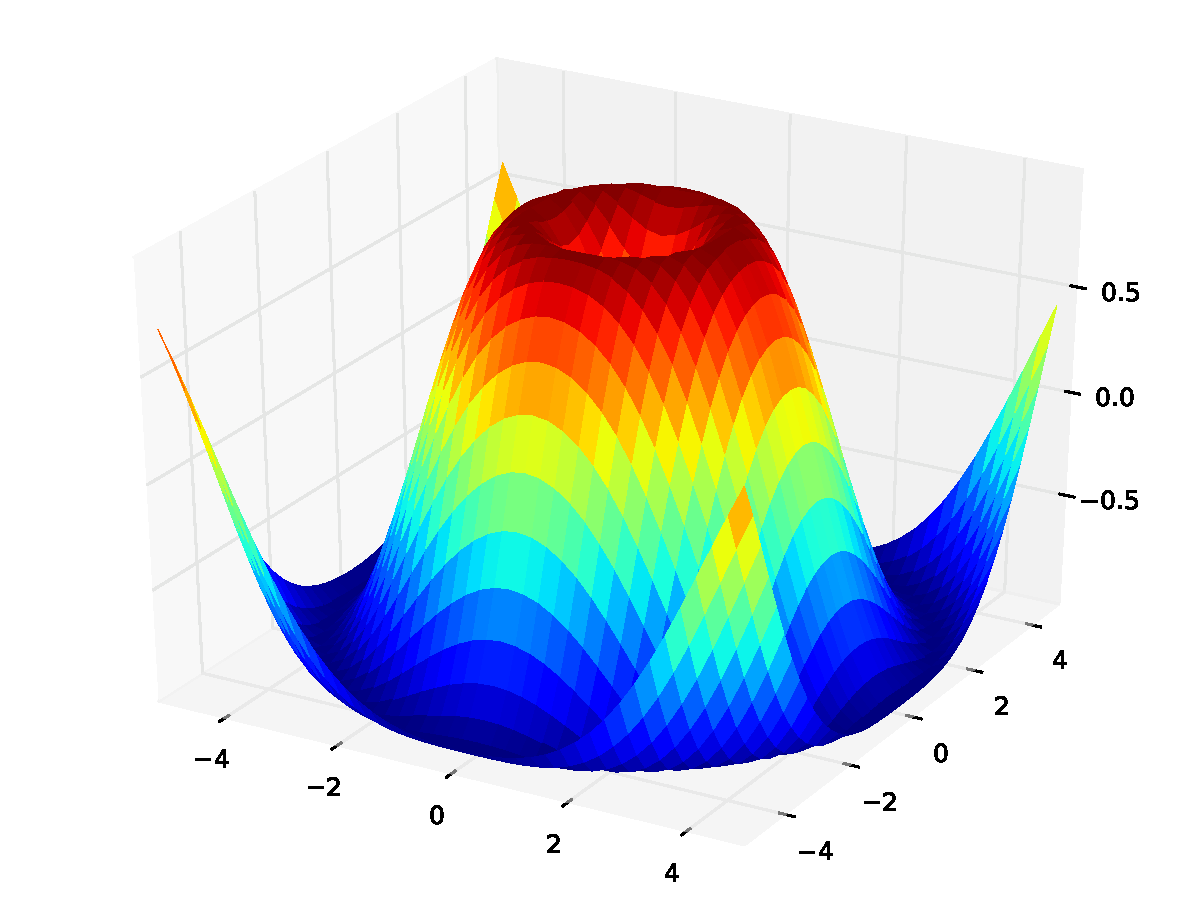
\includegraphics[width=0.6\textwidth]{Chapter-2/figs/threed}
  \caption{A figure in the appendix.}
  \label{fig:app}
\end{figure}
%
\lipsum[7-10]
\begin{table}
  \caption{A table in the appendix.}
  \label{tab:app}
  \begin{center}
    \begin{tabular}{lc}
      \toprule
      System & Author \\
      \midrule
      \TeX   & Donald Knuth   \\
      \LaTeX & Leslie Lamport \\
      \bottomrule
    \end{tabular}
  \end{center}
\end{table}
%

\section{A Second Section}

\lipsum[14-15]


\restoregeometry

%%---------------------------------------------------------------------------%%
%\ensureoddstart
\backmatter


\end{document}
